\documentclass[Main.tex]{subfiles}
\begin{document}
	%%%Phần mở đầu
%	\tatloigiai
	\setcounter{chapter}{5}
	\chapter{Động hóa học}
	\section{Tốc độ phản ứng hóa học}
	\begin{Muctieu}
		\begin{itemize}
			\item Trình bày được khái niệm tốc độ phản ứng và tốc độ phản ứng trung bình.
			\item Phát biểu và vận dụng được định luật tác dụng khối lượng.
			\item Nêu và giải thích được ảnh hưởng của các yếu tố: nồng độ, áp suất, nhiệt độ, diện tích bề mặt, chất xúc tác đến tốc độ phản ứng.
		\end{itemize}
	\end{Muctieu}
	\begin{kd}
		\immini{Quan sát sự khác biệt về thời gian xảy ra của các phản ứng hóa học khác nhau (ví dụ: phản ứng đốt cháy và phản ứng gỉ sắt). Điều gì quyết định sự nhanh chậm của một phản ứng?}{
\includegraphics[width=5cm]{Images/anhhoahoc10/TOCDOPU/PHAN_UNG_TAO_GI.png}\hspace{0.3cm}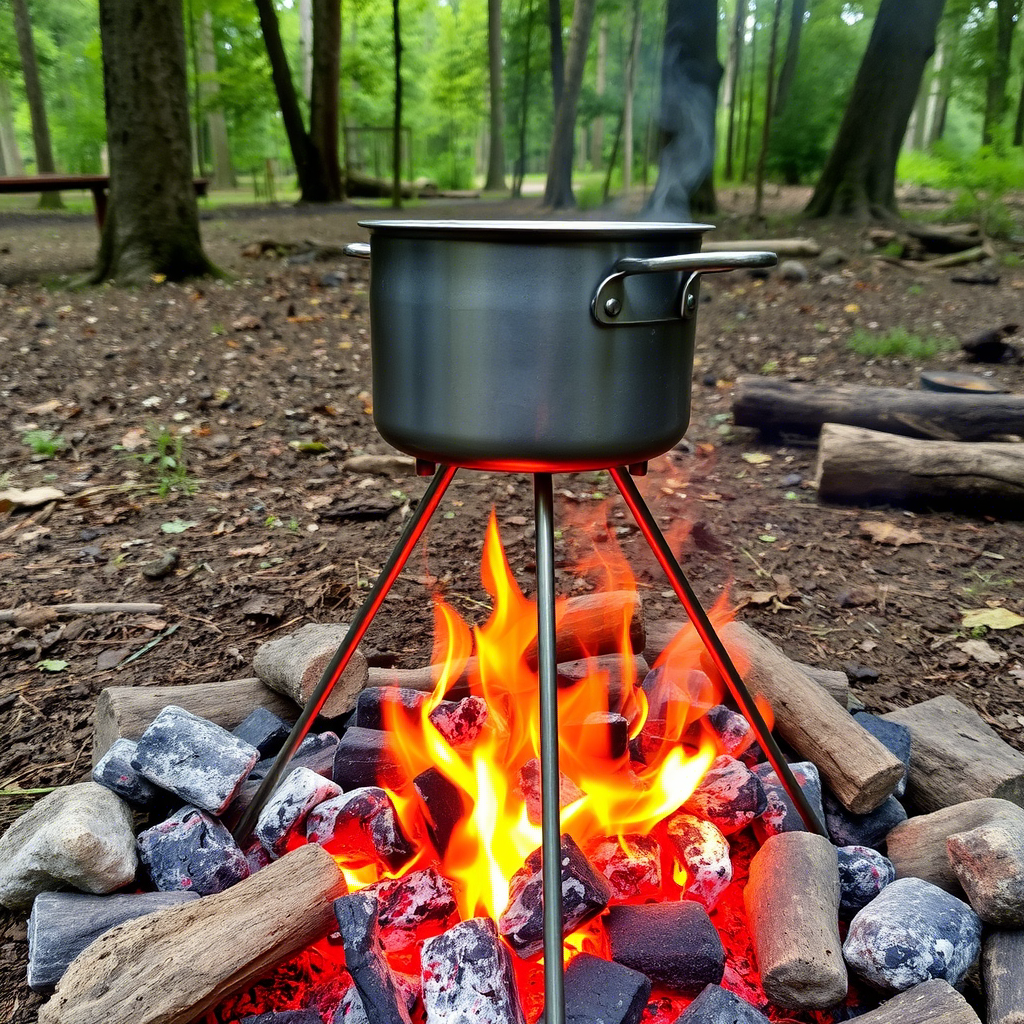
\includegraphics[width=5cm]{Images/anhhoahoc10/TOCDOPU/PHAN_UNG_CHAY.png} }
	\end{kd}
	\subsection{Nội dung bài học}
	\subsubsection{Khái niệm tốc độ phản ứng, tốc độ phản ứng trung bình}
	\Noibat[\maunhan][][][]{Tốc độ phản ứng}
	\begin{ghinho}
	Tốc độ phản ứng của một phản ứng hoá học là đại lượng đặc trưng cho sự thay đổi nồng độ của chất phản ứng hoặc sản phẩm phản ứng trong một đơn vị thời gian.
	\end{ghinho}
	\Noibat[\maunhan][][][]{Tốc độ phản ứng trung bình}
	\begin{ghinho}
		Tốc độ phản ứng trung bình được tính bằng sự thay đổi nồng độ của một chất trong một khoảng thời gian nhất định, chia cho khoảng thời gian đó.
		\[v_{tb} = \frac{\Delta C}{\Delta t}\]
		trong đó: 
		\begin{itemize}
			\item $\Delta C$ là độ biến thiên nồng độ,
			\item $\Delta t$ là khoảng thời gian.
		\end{itemize}
		Đối với phản ứng: $aA + bB \rightarrow cC + dD$, tốc độ phản ứng trung bình được tính theo công thức:
		\[v_{tb} = -\frac{1}{a}\frac{\Delta [A]}{\Delta t} = -\frac{1}{b}\frac{\Delta [B]}{\Delta t} = \frac{1}{c}\frac{\Delta [C]}{\Delta t} = \frac{1}{d}\frac{\Delta [D]}{\Delta t}\]
		\begin{itemize}
			\item Dấu âm (-) thể hiện sự giảm nồng độ của chất phản ứng
			\item Dấu dương (+) thể hiện sự tăng nồng độ của sản phẩm.
		\end{itemize}
	\end{ghinho}
	\subsubsection{Định luật tác dụng khối lượng, hệ số nhiệt Van't Hoff}
	\Noibat[\maunhan][][][]{Định luật tác dụng khối lượng }
	\begin{ghinho}
		Định luật tác dụng khối lượng phát biểu rằng tốc độ phản ứng tỉ lệ thuận với tích nồng độ của các chất phản ứng, với số mũ là hệ số tỉ lượng của chúng trong phương trình hóa học.
		
		Đối với phản ứng: $aA + bB \rightarrow cC + dD$, biểu thức tốc độ phản ứng có dạng: 
		\[\Large \hopcttoan[\maunhan]{v = k[A]^a[B]^b}\]
		trong đó k là hằng số tốc độ phản ứng.
	\end{ghinho}
	\Noibat[\maunhan][][][]{Hệ số nhiệt Van't Hoff}
	\begin{ghinho}
		Hệ số nhiệt Van't Hoff ($\gamma$) cho biết tốc độ phản ứng tăng lên bao nhiêu lần khi nhiệt độ tăng lên $10^\circ C$.
		\[\Large \hopcttoan[\maunhan]{v_{T_2} = v_{T_1} \cdot \gamma^{\frac{T_2 - T_1}{10}}}\]
		trong đó $v_{T_1}$ và $v_{T_2}$ là tốc độ phản ứng ở nhiệt độ $T_1$ và $T_2$.
	\end{ghinho}
	\begin{tomtat}
		\begin{itemize}
			\item \textbf{Định luật tác dụng khối lượng:} $v = k[A]^a[B]^b$ 
			\item \textbf{Hệ số nhiệt Van't Hoff:} $v_{T_2} = v_{T_1} \cdot \gamma^{\frac{T_2 - T_1}{10}}$
		\end{itemize}
	\end{tomtat}
	\subsubsection{Các yếu tố ảnh hưởng đến tốc độ phản ứng}
	\Noibat[\maunhan][][][]{Ảnh hưởng của nồng độ}
	\begin{ghinho}
		Khi tăng nồng độ của chất phản ứng, tốc độ phản ứng tăng lên.
		
		Do tăng nồng độ làm tăng số va chạm hiệu quả giữa các phân tử chất phản ứng.
	\end{ghinho}
	\Noibat[\maunhan][][][]{Ảnh hưởng của ap suất}
	\begin{ghinho}
		Đối với phản ứng có chất khí, khi tăng áp suất, tốc độ phản ứng tăng lên.
		
		Tăng áp suất làm tăng nồng độ của chất khí, do đó làm tăng tốc độ phản ứng.
	\end{ghinho}
	\Noibat[\maunhan][][][]{Ảnh hưởng của nhiệt độ }
	\begin{ghinho}
		Khi tăng nhiệt độ, tốc độ phản ứng tăng lên.
		
		Tăng nhiệt độ làm tăng động năng của các phân tử, làm tăng số va chạm hiệu quả và năng lượng hoạt hóa.
	\end{ghinho}
	\Noibat[\maunhan][][][]{Ảnh hưởng của diện tích bề mặt}
	\begin{ghinho}
		 Đối với phản ứng có chất rắn, khi tăng diện tích bề mặt tiếp xúc, tốc độ phản ứng tăng lên.
		
		Tăng diện tích bề mặt làm tăng số lượng phân tử chất rắn tiếp xúc với chất phản ứng khác.
	\end{ghinho}
	\Noibat[\maunhan][][][]{Ảnh hưởng của chất xúc tác}
	\begin{ghinho}
		Chất xúc tác làm tăng tốc độ phản ứng mà không bị tiêu thụ trong quá trình phản ứng.
		
		Chất xúc tác làm giảm năng lượng hoạt hóa của phản ứng, tạo điều kiện cho phản ứng xảy ra dễ dàng hơn.
	\end{ghinho}
	\begin{tomtat}
		\textbf{Tăng tốc độ phản ứng:} Tăng nồng độ, áp suất (đối với khí), nhiệt độ, diện tích bề mặt; sử dụng chất xúc tác.
	\end{tomtat}
	\subsection{Bài tập}
	\begin{dang}{Tính tốc độ phản ứng trung bình}
	\end{dang}
	\begin{phuongphap}
		Xét phản ứng : $aA + bB \rightarrow cC + dD$
		\begin{cacbuoc}
			\item Xác định nồng độ ban đầu và nồng độ sau thời gian $\Delta t$.
			\item Tính độ biến thiên nồng độ $\Delta C$.
			\item Áp dụng công thức để tính $v_{tb}$.
			\[v_{tb} = -\frac{1}{a}\frac{\Delta [A]}{\Delta t} = -\frac{1}{b}\frac{\Delta [B]}{\Delta t} = \frac{1}{c}\frac{\Delta [C]}{\Delta t} = \frac{1}{d}\frac{\Delta [D]}{\Delta t}\]
			\begin{itemize}
				\item Dấu âm (-) áp dụng cho chất tham gia
				\item Dấu dương (+) áp dụng cho chất sản phẩm.
			\end{itemize}
		\end{cacbuoc}
	\end{phuongphap}
	\Noibat[\maunhan][][\faBookmark][]{Ví dụ mẫu}
	\begin{vd}
		Cho phản ứng: $2N_2O_5(g) \rightarrow 4NO_2(g) + O_2(g)$. Nồng độ ban đầu của $N_2O_5$ là 0.5M, sau 10 phút nồng độ còn lại là 0.4M. Tính tốc độ phản ứng trung bình của phản ứng trên.
		\choice
		{$0.001$ \, \text{M/phút}}
		{$0.05$ \, \text{M/phút}}
		{\True $0.005$ \, \text{M/phút}}
		{$0.01$ \, \text{M/phút}}
		\loigiai{
		\begin{eqnarray*}
				\Delta [N_2O_5] &=& 0.4 - 0.5 = -0.1 M \\
			\Rightarrow v_{tb} &=& -\frac{1}{2} \frac{\Delta [N_2O_5]}{\Delta t} = -\frac{1}{2} \frac{-0.1}{10} = 0.005\, \text{M/phút}
		\end{eqnarray*}
		}
	\end{vd}
	
	%%%%%=====================Bài tập tự luyện Dạng 1==========================%%%
	\Noibat[\maunhan][][\faBook][]{Bài tập tự luyện}
	
	\phan{Bài tập tự luận}
	%%%=============SOẠN BT===============%%%
	\Opensolutionfile{ansbth}[Ans/LGBT-C06B01_Dang1]
	\Opensolutionfile{ansbt}[Ans/AnsBT-C06B01_Dang1]
	%%%=============BT_01=============%%%
	\begin{bt}
		Xét phản ứng: $N_2(g) + 3H_2(g) \rightarrow 2NH_3(g)$.
		Nồng độ ban đầu của $N_2$ là $0{,}10 M$. Sau $10$ phút, nồng độ của $N_2$ là $0{,}08 M$. Tính tốc độ trung bình của phản ứng trong khoảng thời gian trên theo $NH_3$.
		\loigiai{
			Tốc độ trung bình của phản ứng:
			\[v = -\frac{\Delta [N_2]}{\Delta t} = \frac{1}{2} \frac{\Delta [NH_3]}{\Delta t}\]
			\[\Delta [NH_3] = 2 \times (-\Delta [N_2]) = 2 \times (0{,}10 - 0{,}08) = 0{,}04 M\]
			\[v_{tb} = \frac{\Delta [NH_3]}{\Delta t} = \frac{0{,}04}{10} = 0{,}004 M/phút\]
		}
	\end{bt}
	
	%%%=============BT_02=============%%%
	\begin{bt}
		Cho phản ứng: $2SO_2(g) + O_2(g) \rightarrow 2SO_3(g)$.
		Nồng độ ban đầu của $SO_2$ là $0{,}05 M$. Sau $20$ giây, nồng độ của $SO_2$ là $0{,}04 M$. Tính tốc độ trung bình của phản ứng trong khoảng thời gian trên theo $O_2$.
		\loigiai{
			Tốc độ trung bình của phản ứng:
			\[v = -\frac{1}{2} \frac{\Delta [SO_2]}{\Delta t} = -\frac{\Delta [O_2]}{\Delta t}\]
			\[\Delta [O_2] = \frac{1}{2} \Delta [SO_2] = \frac{1}{2} (0{,}05 - 0{,}04) = 0{,}005 M\]
			\[v_{tb} = -\frac{\Delta [O_2]}{\Delta t} = \frac{0{,}005}{20} = 2{,}5 \times 10^{-4} M/s\]
		}
	\end{bt}
	
	%%%=============BT_03=============%%%
	\begin{bt}
		Xét phản ứng: $H_2(g) + I_2(g) \rightarrow 2HI(g)$.
		Nồng độ ban đầu của $H_2$ là $0{,}01 M$. Sau $30$ giây, nồng độ của $HI$ là $0{,}015 M$. Tính tốc độ trung bình của phản ứng trong khoảng thời gian trên theo $H_2$.
		\loigiai{
			Tốc độ trung bình của phản ứng:
			\[v = -\frac{\Delta [H_2]}{\Delta t} = \frac{1}{2} \frac{\Delta [HI]}{\Delta t}\]
			\[\Delta [H_2] = -\frac{1}{2} \Delta [HI] = -\frac{1}{2} (0{,}015 - 0) = -0{,}0075 M\]
			\[v_{tb} = -\frac{\Delta [H_2]}{\Delta t} = \frac{0{,}0075}{30} = 2{,}5 \times 10^{-4} M/s\]
		}
	\end{bt}
	
	%%%=============BT_04=============%%%
	\begin{bt}
		Cho phản ứng: $2NO(g) + Cl_2(g) \rightarrow 2NOCl(g)$.
		Nồng độ ban đầu của $NO$ là $0{,}03 M$. Sau $40$ giây, nồng độ của $NOCl$ là $0{,}01 M$. Tính tốc độ trung bình của phản ứng trong khoảng thời gian trên theo $Cl_2$.
		\loigiai{
			Tốc độ trung bình của phản ứng:
			\[v = -\frac{1}{2} \frac{\Delta [NO]}{\Delta t} = -\frac{\Delta [Cl_2]}{\Delta t} = \frac{1}{2} \frac{\Delta [NOCl]}{\Delta t}\]
			\[\Delta [Cl_2] = -\frac{1}{2} \Delta [NOCl] = -\frac{1}{2} (0{,}01 - 0) = -0{,}005 M\]
			\[v_{tb} = -\frac{\Delta [Cl_2]}{\Delta t} = \frac{0{,}005}{40} = 1{,}25 \times 10^{-4} M/s\]
		}
	\end{bt}
	
	%%%=============BT_05=============%%%
	\begin{bt}
		Xét phản ứng: $C_2H_4(g) + H_2(g) \rightarrow C_2H_6(g)$.
		Nồng độ ban đầu của $C_2H_4$ là $0{,}04 M$. Sau $50$ giây, nồng độ của $C_2H_6$ là $0{,}02 M$. Tính tốc độ trung bình của phản ứng trong khoảng thời gian trên theo $H_2$.
		\loigiai{
			Tốc độ trung bình của phản ứng:
			\[v = -\frac{\Delta [C_2H_4]}{\Delta t} = -\frac{\Delta [H_2]}{\Delta t} = \frac{\Delta [C_2H_6]}{\Delta t}\]
			\[\Delta [H_2] = \Delta [C_2H_4] = (0{,}04 - 0{,}02) = -0{,}02 M\]
			\[v_{tb} = -\frac{\Delta [H_2]}{\Delta t} = \frac{0{,}02}{50} = 4 \times 10^{-4} M/s\]
		}
	\end{bt}
	
	%%%=============BT_06=============%%%
	\begin{bt}
		Cho phản ứng: $2N_2O(g) \rightarrow 2N_2(g) + O_2(g)$.
		Nồng độ ban đầu của $N_2O$ là $0{,}06 M$. Sau $60$ giây, nồng độ của $O_2$ là $0{,}01 M$. Tính tốc độ trung bình của phản ứng trong khoảng thời gian trên theo $N_2O$.
		\loigiai{
			Tốc độ trung bình của phản ứng:
			\[v = -\frac{1}{2} \frac{\Delta [N_2O]}{\Delta t} = \frac{1}{2} \frac{\Delta [N_2]}{\Delta t} = \frac{\Delta [O_2]}{\Delta t}\]
			\[\Delta [N_2O] = -2\Delta [O_2] = -2 (0{,}01 - 0) = -0{,}02 M\]
			\[v_{tb} = -\frac{1}{2} \frac{\Delta [N_2O]}{\Delta t} = \frac{1}{2} \frac{0{,}02}{60} = 1{,}67 \times 10^{-4} M/s\]
		}
	\end{bt}
	
	%%%=============BT_07=============%%%
	\begin{bt}
		Xét phản ứng: $4NH_3(g) + 5O_2(g) \rightarrow 4NO(g) + 6H_2O(g)$.
		Nồng độ ban đầu của $NH_3$ là $0{,}07 M$. Sau $70$ giây, nồng độ của $NO$ là $0{,}03 M$. Tính tốc độ trung bình của phản ứng trong khoảng thời gian trên theo $O_2$.
		\loigiai{
			Tốc độ trung bình của phản ứng:
			\[v = -\frac{1}{4} \frac{\Delta [NH_3]}{\Delta t} = -\frac{1}{5} \frac{\Delta [O_2]}{\Delta t} = \frac{1}{4} \frac{\Delta [NO]}{\Delta t} = \frac{1}{6} \frac{\Delta [H_2O]}{\Delta t}\]
			\[\Delta [O_2] = -\frac{5}{4} \Delta [NO] = -\frac{5}{4} (0{,}03 - 0) = -0{,}0375 M\]
			\[v_{tb} = -\frac{1}{5} \frac{\Delta [O_2]}{\Delta t} = \frac{1}{5} \frac{0{,}0375}{70} = 1{,}07 \times 10^{-4} M/s\]
		}
	\end{bt}
	
	%%%=============BT_08=============%%%
	\begin{bt}
		Cho phản ứng: $2H_2O_2(aq) \rightarrow 2H_2O(l) + O_2(g)$.
		Nồng độ ban đầu của $H_2O_2$ là $0{,}08 M$. Sau $80$ giây, nồng độ của $O_2$ là $0{,}02 M$. Tính tốc độ trung bình của phản ứng trong khoảng thời gian trên theo $H_2O_2$.
		\loigiai{
			Tốc độ trung bình của phản ứng:
			\[v = -\frac{1}{2} \frac{\Delta [H_2O_2]}{\Delta t} = \frac{1}{2} \frac{\Delta [H_2O]}{\Delta t} = \frac{\Delta [O_2]}{\Delta t}\]
			\[\Delta [H_2O_2] = -2\Delta [O_2] = -2 (0{,}02 - 0) = -0{,}04 M\]
			\[v_{tb} = -\frac{1}{2} \frac{\Delta [H_2O_2]}{\Delta t} = \frac{1}{2} \frac{0{,}04}{80} = 2{,}5 \times 10^{-4} M/s\]
		}
	\end{bt}
	
	%%%=============BT_09=============%%%
	\begin{bt}
		Xét phản ứng: $5Br^-(aq) + BrO_3^-(aq) + 6H^+(aq) \rightarrow 3Br_2(aq) + 3H_2O(l)$.
		Nồng độ ban đầu của $Br^-$ là $0{,}09 M$. Sau $90$ giây, nồng độ của $Br_2$ là $0{,}01 M$. Tính tốc độ trung bình của phản ứng trong khoảng thời gian trên theo $BrO_3^-$.
		\loigiai{
			Tốc độ trung bình của phản ứng:
			\[v = -\frac{1}{5} \frac{\Delta [Br^-]}{\Delta t} = -\frac{\Delta [BrO_3^-]}{\Delta t} = \frac{1}{3} \frac{\Delta [Br_2]}{\Delta t} = \frac{1}{3} \frac{\Delta [H_2O]}{\Delta t}\]
			\[\Delta [BrO_3^-] = -\frac{1}{3} \Delta [Br_2] = -\frac{1}{3} (0{,}01 - 0) = -0{,}00333 M\]
			\[v_{tb} = -\frac{\Delta [BrO_3^-]}{\Delta t} = \frac{0{,}00333}{90} = 3{,}7 \times 10^{-5} M/s\]
		}
	\end{bt}
	
	%%%=============BT_10=============%%%
	\begin{bt}
		Cho phản ứng: $C_4H_8 \rightarrow 2C_2H_4$.
		Nồng độ ban đầu của $C_4H_8$ là $0{,}25 M$. Sau $100$ giây, nồng độ của $C_2H_4$ là $0{,}1 M$. Tính tốc độ trung bình của phản ứng trong khoảng thời gian trên theo $C_4H_8$.
		\loigiai{
			Tốc độ trung bình của phản ứng:
			\[v = -\frac{\Delta [C_4H_8]}{\Delta t} = \frac{1}{2} \frac{\Delta [C_2H_4]}{\Delta t}\]
			\[\Delta [C_4H_8] = -\frac{1}{2} \Delta [C_2H_4] = -\frac{1}{2} (0{,}1 - 0) = -0{,}05 M\]
			\[v_{tb} = -\frac{\Delta [C_4H_8]}{\Delta t} = \frac{0{,}05}{100} = 5 \times 10^{-4} M/s\]
		}
	\end{bt}
	\Closesolutionfile{ansbt}
	\Closesolutionfile{ansbth}
	%\bangdapanSA{AnsBT-C06B01_Dang1}
	
	%%%=============SOẠN SA===============%%%
	\Opensolutionfile{ansbth}[Ans/LGSA-C06B01_Dang1]
	\Opensolutionfile{ansbt}[Ans/AnsSA-C06B01_Dang1]
	%%%=============SA_1=============%%%
	\begin{bt}
		Phản ứng $A \rightarrow B$ có tốc độ phản ứng trung bình là $5 \times 10^{-3} \, mol/L.s$. Hỏi sau $20$ giây, nồng độ của $B$ tăng lên bao nhiêu (giả sử nồng độ ban đầu của $B$ là $0$)?
		\shortans{$0,1$}
		\loigiai{
			\[\Delta [B] = v \times \Delta t = 5 \times 10^{-3} \times 20 = 0{,}1 \, mol/L\]
		}
	\end{bt}
	
	%%%=============SA_2=============%%%
	\begin{bt}
		Cho phản ứng $2A \rightarrow B$. Tốc độ phản ứng trung bình là $2{,}5 \times 10^{-4} \, mol/L.phút$. Hỏi sau $30$ phút, nồng độ của $A$ giảm đi bao nhiêu?
		\shortans{$0,015$}
		\loigiai{
			\[-\Delta [A] = 2 \times v \times \Delta t = 2 \times 2{,}5 \times 10^{-4} \times 30 = 0{,}015 \, mol/L\]
		}
	\end{bt}
	
	%%%=============SA_3=============%%%
	\begin{bt}
		Phản ứng $A + B \rightarrow C$ có tốc độ phản ứng trung bình là $1{,}2 \times 10^{-2} \, mol/L.s$. Hỏi sau $15$ giây, nồng độ của $C$ tăng lên bao nhiêu (giả sử nồng độ ban đầu của $C$ là $0$)?
		\shortans{0.18}
		\loigiai{
			\[\Delta [C] = v \times \Delta t = 1{,}2 \times 10^{-2} \times 15 = 0{,}18 \, mol/L\]
		}
	\end{bt}
	
	%%%=============SA_4=============%%%
	\begin{bt}
		Cho phản ứng $A \rightarrow B + C$. Tốc độ phản ứng trung bình là $8 \times 10^{-5} \, mol/L.phút$. Hỏi sau $1$ giờ, nồng độ của $B$ tăng lên bao nhiêu?
		\shortans{0.0048}
		\loigiai{
			\[\Delta [B] = v \times \Delta t = 8 \times 10^{-5} \times 60 = 0{,}0048 \, mol/L\]
		}
	\end{bt}
	
	%%%=============SA_5=============%%%
	\begin{bt}
		Phản ứng $2A + B \rightarrow C$ có tốc độ phản ứng trung bình là $3 \times 10^{-3} \, mol/L.s$. Hỏi sau $10$ giây, nồng độ của $A$ giảm đi bao nhiêu?
		\shortans{0.06}
		\loigiai{
			\[-\Delta [A] = 2 \times v \times \Delta t = 2 \times 3 \times 10^{-3} \times 10 = 0{,}06 \, mol/L\]
		}
	\end{bt}
	
	%%%=============SA_6=============%%%
	\begin{bt}
		Cho phản ứng $A \rightarrow 2B$. Tốc độ phản ứng trung bình là $4{,}5 \times 10^{-4} \, mol/L.phút$. Hỏi sau $2$ giờ, nồng độ của $B$ tăng lên bao nhiêu?
		\shortans{0.054}
		\loigiai{
			\[\Delta [B] = 2 \times v \times \Delta t = 2 \times 4{,}5 \times 10^{-4} \times 120 = 0{,}108 \, mol/L\]
		}
	\end{bt}
	
	%%%=============SA_7=============%%%
	\begin{bt}
		Phản ứng $A + 2B \rightarrow C$ có tốc độ phản ứng trung bình là $6 \times 10^{-2} \, mol/L.s$. Hỏi sau $5$ giây, nồng độ của $B$ giảm đi bao nhiêu?
		\shortans{0.6}
		\loigiai{
			\[-\Delta [B] = 2 \times v \times \Delta t = 2 \times 6 \times 10^{-2} \times 5 = 0{,}6 \, mol/L\]
		}
	\end{bt}
	
	%%%=============SA_8=============%%%
	\begin{bt}
		Cho phản ứng $3A \rightarrow B$. Tốc độ phản ứng trung bình là $1{,}5 \times 10^{-4} \, mol/L.phút$. Hỏi sau $45$ phút, nồng độ của $A$ giảm đi bao nhiêu?
		\shortans{0.02025}
		\loigiai{
			\[-\Delta [A] = 3 \times v \times \Delta t = 3 \times 1{,}5 \times 10^{-4} \times 45 = 0{,}02025 \, mol/L\]
		}
	\end{bt}
	
	%%%=============SA_9=============%%%
	\begin{bt}
		Phản ứng $A \rightarrow B + 2C$ có tốc độ phản ứng trung bình là $2{,}0 \times 10^{-3} \, mol/L.s$. Hỏi sau $30$ giây, nồng độ của $C$ tăng lên bao nhiêu?
		\shortans{0.12}
		\loigiai{
			\[\Delta [C] = 2 \times v \times \Delta t = 2 \times 2{,}0 \times 10^{-3} \times 30 = 0{,}12 \, mol/L\]
		}
	\end{bt}
	
	%%%=============SA_10=============%%%
	\begin{bt}
		Cho phản ứng $4A \rightarrow B$. Tốc độ phản ứng trung bình là $7{,}5 \times 10^{-5} \, mol/L.phút$. Hỏi sau $2$ giờ, nồng độ của $A$ giảm đi bao nhiêu?
		\shortans{0.036}
		\loigiai{
			\[-\Delta [A] = 4 \times v \times \Delta t = 4 \times 7{,}5 \times 10^{-5} \times 120 = 0{,}036 \, mol/L\]
		}
	\end{bt}
	\Closesolutionfile{ansbt}
	\Closesolutionfile{ansbth}
	%\bangdapanSA{AnsSA-C06B01_Dang1}
	
	
	%%%%============Phần trắc nghiệm============%%%
	\phan{Trắc nghiệm nhiều lựa chọn}
	%%%=============SOẠN EX===============%%%
	\Opensolutionfile{ansex}[Ans/LGEX-C06B01_Dang1]
	\Opensolutionfile{ans}[Ans/Ans-C06B01_Dang1]
	%%%=============EX_01================%%%%
	\begin{ex}
		Cho phản ứng: $2N_2O_5(g) \rightarrow 4NO_2(g) + O_2(g)$. Nồng độ ban đầu của $N_2O_5$ là $0{,}500M$. Sau $500$ giây, nồng độ của $N_2O_5$ là $0{,}400M$. Tốc độ phản ứng trung bình trong khoảng thời gian này là:
		\choice
		{$2{,}0 \times 10^{-4} M/s$}
		{$4{,}0 \times 10^{-4} M/s$}
		{\True $1{,}0 \times 10^{-4} M/s$}
		{$8{,}0 \times 10^{-4} M/s$}
		\loigiai{Tốc độ phản ứng trung bình: $v = -\frac{1}{2} \frac{\Delta [N_2O_5]}{\Delta t} = -\frac{1}{2} \frac{0{,}400 - 0{,}500}{500} = 1{,}0 \times 10^{-4} M/s$}
	\end{ex}
	
	%%%=============EX_02================%%%%
	\begin{ex}
		Cho phản ứng: $A \rightarrow B$. Sau $10$ phút, nồng độ chất $A$ giảm từ $0{,}8M$ xuống $0{,}4M$. Tốc độ phản ứng trung bình là:
		\choice
		{$0{,}08 \, \text{M/phút}$}
		{$0{,}02 \, \text{M/phút}$}
		{$0{,}8 \, \text{M/phút}$}
		{\True $0{,}04 \, \text{M/phút}$}
		\loigiai{Tốc độ phản ứng trung bình: $v = -\frac{\Delta [A]}{\Delta t} = -\frac{0{,}4 - 0{,}8}{10} = 0{,}04 \, \text{M/phút}$}
	\end{ex}
	
	%%%=============EX_03================%%%%
	\begin{ex}
		Cho phản ứng: $2A + B \rightarrow C$. Nồng độ ban đầu của $A$ là $1{,}0M$. Sau $2$ phút, nồng độ của $A$ là $0{,}6M$. Tốc độ phản ứng trung bình theo chất $A$ là:
		\choice
		{$0{,}4 \, \text{M/phút}$}
		{$0{,}1 \, \text{M/phút}$}
		{$0{,}8 \, \text{M/phút}$}
		{\True $0{,}2 \, \text{M/phút}$}
		\loigiai{Tốc độ phản ứng trung bình: $v = -\frac{1}{2} \frac{\Delta [A]}{\Delta t} = -\frac{1}{2} \frac{0{,}6 - 1{,}0}{2} = 0{,}1 \, \text{M/phút}$}
	\end{ex}
	
	%%%=============EX_04================%%%%
	\begin{ex}
		Cho phản ứng: $A + 2B \rightarrow C$. Nồng độ ban đầu của $B$ là $2{,}0M$. Sau $5$ phút, nồng độ của $B$ là $1{,}0M$. Tốc độ phản ứng trung bình theo chất $C$ là:
		\choice
		{$0{,}1 \, \text{M/phút}$}
		{$0{,}4 \, \text{M/phút}$}
		{\True $0{,}1 \, \text{M/phút}$}
		{$0{,}2 \, \text{M/phút}$}
		\loigiai{Tốc độ phản ứng trung bình: $v = \frac{\Delta [C]}{\Delta t} = -\frac{1}{2} \frac{\Delta [B]}{\Delta t} = -\frac{1}{2} \frac{1{,}0 - 2{,}0}{5} = 0{,}1 \, \text{M/phút}$}
	\end{ex}
	
	%%%=============EX_05================%%%%
	\begin{ex}
		Cho phản ứng: $A \rightarrow 2B + C$. Nồng độ chất $A$ giảm từ $0{,}5M$ xuống $0{,}2M$ trong $3$ phút. Tốc độ phản ứng trung bình theo chất $B$ là:
		\choice
		{\True $0{,}1 \, \text{M/phút}$}
		{$0{,}6 \, \text{M/phút}$}
		{$0{,}2 \, \text{M/phút}$}
		{ $0{,}2 \, \text{M/phút}$}
		\loigiai{Tốc độ phản ứng trung bình: $v = -\frac{1}{2} \frac{\Delta [B]}{\Delta t} = -\frac{\Delta [A]}{\Delta t} = -\frac{0{,}2 - 0{,}5}{3} = 0{,}1 \, \text{M/phút}$}
	\end{ex}
	
	%%%=============EX_06================%%%%
	\begin{ex}
		Phản ứng $X \rightarrow Y$ có nồng độ $X$ giảm từ $0{,}6M$ xuống $0{,}3M$ trong $15$ giây. Tốc độ trung bình của phản ứng là:
		\choice
		{$0{,}01 M/s$}
		{$0{,}04 M/s$}
		{$0{,}03 M/s$}
		{\True $0{,}02 M/s$}
		\loigiai{Tốc độ trung bình: $v = -\frac{\Delta [X]}{\Delta t} = -\frac{0{,}3 - 0{,}6}{15} = 0{,}02 M/s$}
	\end{ex}
	
	%%%=============EX_07================%%%%
	\begin{ex}
		Cho phản ứng: $A + B \rightarrow C + D$. Nồng độ $A$ giảm $0{,}2M$ trong $4$ phút. Tốc độ trung bình của phản ứng là:
		\choice
		{$0{,}02 \, \text{M/phút}$}
		{$0{,}01 \, \text{M/phút}$}
		{\True $0{,}05 \, \text{M/phút}$}
		{$0{,}08 \, \text{M/phút}$}
		\loigiai{Tốc độ trung bình: $v = -\frac{\Delta [A]}{\Delta t} = -\frac{-0{,}2}{4} = 0{,}05 \, \text{M/phút}$}
	\end{ex}
	
	%%%=============EX_08================%%%%
	\begin{ex}
		Cho phản ứng: $A \rightarrow B + C$. Nồng độ $B$ tăng từ $0M$ lên $0{,}6M$ trong $6$ phút. Tốc độ trung bình của phản ứng là:
		\choice
		{$0{,}2 \, \text{M/phút}$}
		{\True $0{,}1 \, \text{M/phút}$}
		{$0{,}3 \, \text{M/phút}$}
		{$0{,}4 \, \text{M/phút}$}
		\loigiai{Tốc độ trung bình: $v = \frac{\Delta [B]}{\Delta t} = \frac{0{,}6 - 0}{6} = 0{,}1 \, \text{M/phút}$}
	\end{ex}
	
	%%%=============EX_09================%%%%
	\begin{ex}
		Cho phản ứng: $A + B \rightarrow C$. Nồng độ $C$ tăng từ $0M$ lên $0{,}4M$ trong $8$ phút. Tốc độ trung bình của phản ứng là:
		\choice
		{$0{,}02 \, \text{M/phút}$}
		{$0{,}08 \, \text{M/phút}$}
		{$0{,}03 \, \text{M/phút}$}
		{\True $0{,}05 \, \text{M/phút}$}
		\loigiai{Tốc độ trung bình: $v = \frac{\Delta [C]}{\Delta t} = \frac{0{,}4 - 0}{8} = 0{,}05 \, \text{M/phút}$}
	\end{ex}
	
	%%%=============EX_10================%%%%
	\begin{ex}
		Cho phản ứng: $A \rightarrow B$. Nồng độ $A$ giảm từ $1{,}2M$ xuống $0{,}9M$ trong $30$ giây. Tốc độ trung bình của phản ứng là:
		\choice
		{$0{,}02 M/s$}
		{$0{,}01 M/s$}
		{\True $0{,}01 M/s$}
		{$0{,}04 M/s$}
		\loigiai{Tốc độ trung bình: $v = -\frac{\Delta [A]}{\Delta t} = -\frac{0{,}9 - 1{,}2}{30} = 0{,}01 M/s$}
	\end{ex}
	
	%%%=============EX_11================%%%%
	\begin{ex}
		Cho phản ứng: $A + B \rightarrow C$. Nếu nồng độ của $A$ giảm từ $0{,}50 M$ xuống $0{,}25 M$ trong 100 giây, tốc độ trung bình của phản ứng là:
		\choice
		{$0{,}0050 M/s$}
		{\True $0{,}0025 M/s$}
		{$0{,}0075 M/s$}
		{$0{,}00125 M/s$}
		\loigiai{Tốc độ trung bình: $v = -\frac{\Delta [A]}{\Delta t} = -\frac{0{,}25 - 0{,}50}{100} = 0{,}0025 M/s$}
	\end{ex}
	
	%%%=============EX_12================%%%%
	\begin{ex}
		Cho phản ứng: $2A \rightarrow B$. Nếu nồng độ của $A$ giảm từ $1{,}0 M$ xuống $0{,}5 M$ trong 5 phút, tốc độ trung bình của phản ứng tính theo $A$ là:
		\choice
		{$0{,}1 \, \text{M/phút}$}
		{$0{,}05 \, \text{M/phút}$}
		{\True $0{,}05 \, \text{M/phút}$}
		{$0{,}2 \, \text{M/phút}$}
		\loigiai{Tốc độ trung bình: $v = -\frac{1}{2}\frac{\Delta [A]}{\Delta t} = -\frac{1}{2} \frac{0{,}5 - 1{,}0}{5} = 0{,}05 \, \text{M/phút}$}
	\end{ex}
	
	%%%=============EX_13================%%%%
	\begin{ex}
		Cho phản ứng: $A + 2B \rightarrow C$. Nếu nồng độ của $B$ giảm từ $2{,}0 M$ xuống $1{,}5 M$ trong 10 phút, tốc độ trung bình của phản ứng tính theo $C$ là:
		\choice
		{$0{,}1 \, \text{M/phút}$}
		{\True $0{,}025 \, \text{M/phút}$}
		{$0{,}05 \, \text{M/phút}$}
		{$0{,}2 \, \text{M/phút}$}
		\loigiai{Tốc độ trung bình: $v = \frac{\Delta [C]}{\Delta t} = -\frac{1}{2}\frac{\Delta [B]}{\Delta t} = -\frac{1}{2} \frac{1{,}5 - 2{,}0}{10} = 0{,}025 \, \text{M/phút}$}
	\end{ex}
	
	%%%=============EX_14================%%%%
	\begin{ex}
		Cho phản ứng: $A \rightarrow 3C$. Nếu nồng độ của $A$ giảm từ $0{,}8 M$ xuống $0{,}2 M$ trong 2 phút, tốc độ trung bình của phản ứng tính theo $C$ là:
		\choice
		{$0{,}3 \, \text{M/phút}$}
		{$0{,}6 \, \text{M/phút}$}
		{\True $0{,}9 \, \text{M/phút}$}
		{$0{,}1 \, \text{M/phút}$}
		\loigiai{Tốc độ trung bình: $v = 3\frac{\Delta [C]}{\Delta t} = -\frac{\Delta [A]}{\Delta t} \implies \frac{\Delta [C]}{\Delta t} = -\frac{1}{3} \frac{\Delta [A]}{\Delta t} = -\frac{1}{3} \frac{0{,}2 - 0{,}8}{2} = 0{,}1 \, \text{M/phút}$}
	\end{ex}
	
	%%%=============EX_15================%%%%
	\begin{ex}
		Cho phản ứng: $2A + B \rightarrow 2D$. Nếu nồng độ của $B$ giảm từ $0{,}6 M$ xuống $0{,}4 M$ trong 4 phút, tốc độ trung bình của phản ứng tính theo $D$ là:
		\choice
		{$0{,}05 \, \text{M/phút}$}
		{\True $0{,}1 \, \text{M/phút}$}
		{$0{,}2 \, \text{M/phút}$}
		{$0{,}4 \, \text{M/phút}$}
		\loigiai{Tốc độ trung bình: $v = 2\frac{\Delta [D]}{\Delta t} = -\frac{\Delta [B]}{\Delta t} \Rightarrow \frac{\Delta [D]}{\Delta t} = -\frac{1}{2} \frac{\Delta [B]}{\Delta t} = -\frac{1}{2} \frac{0{,}4 - 0{,}6}{4} = 0{,}025 \, \text{M/phút}$}
	\end{ex}
	\Closesolutionfile{ans}
	\Closesolutionfile{ansex}
	%\bangdapan{Ans-C02B01_Dang1}
	
%	%%%%%%%%%%%%%%%Trắc nghiệm đúng sai%%%%%%%%%%%%%%%%%%%%%%%%
%	\phan{Bài tập trắc nghiệm Đúng Sai}
%	%%%=============SOẠN EXTF===============%%%
%	\Opensolutionfile{ansex}[Ans/LGTF-C06B01_Dang1]
%	\Opensolutionfile{ansbook}[Ansbook/AnsTF-C06B01_Dang1]
%	\Opensolutionfile{ans}[Ans/Tempt-C06B01_Dang1]
%	\begin{ex}%[0C1Y1-1]
%		Xét các phát biểu sau:
%		\choiceTF
%		{\True Tốc độ phản ứng tỉ lệ thuận với nồng độ chất phản ứng.}
%		{Chất xúc tác làm giảm tốc độ phản ứng.}
%		{\True Nhiệt độ tăng làm tăng tốc độ phản ứng.}
%		{Diện tích bề mặt không ảnh hưởng đến tốc độ phản ứng của chất rắn.}
%		\loigiai{
%			\begin{itemchoice}[T1,F2,T3,F4]
%				\itemch Tăng nồng độ làm tăng số va chạm hiệu quả.
%				\itemch Chất xúc tác làm tăng tốc độ phản ứng.
%				\itemch Tăng nhiệt độ làm tăng động năng của phân tử.
%				\itemch Diện tích bề mặt lớn hơn làm tăng số lượng phân tử tiếp xúc.
%			\end{itemchoice}
%		}
%	\end{ex}
%	\Closesolutionfile{ans}
%	\Closesolutionfile{ansbook}
%	\Closesolutionfile{ansex}
%	%\bangdapanTF{AnsTF-C06B01_Dang1}
%%%=====================Dạng 2================%%%
\begin{dang}{Viết biểu thức tính tốc độ phản ứng}
\end{dang}
\phan{Trắc nghiệm nhiều lựa chọn}
%%%=============SOẠN EX===============%%%
\Opensolutionfile{ansex}[Ans/LGEX-C06B01_Dang2]
\Opensolutionfile{ans}[Ans/Ans-C06B01_Dang2]
	%%%=============EX_01================%%%%
	\begin{ex}
		Cho phản ứng: $N_2(g) + 3H_2(g) \rightarrow 2NH_3(g)$. Biểu thức tốc độ trung bình của phản ứng là:
		\choice
		{$v = \frac{\Delta [N_2]}{\Delta t} = \frac{\Delta [H_2]}{3\Delta t} = \frac{\Delta [NH_3]}{2\Delta t}$}
		{$v = -\frac{\Delta [N_2]}{\Delta t} = -\frac{\Delta [H_2]}{3\Delta t} = \frac{\Delta [NH_3]}{2\Delta t}$}
		{$v = -\frac{\Delta [N_2]}{\Delta t} = -\frac{\Delta [H_2]}{\Delta t} = \frac{\Delta [NH_3]}{\Delta t}$}
		{\True $v = -\frac{\Delta [N_2]}{\Delta t} = -\frac{1}{3}\frac{\Delta [H_2]}{\Delta t} = \frac{1}{2}\frac{\Delta [NH_3]}{\Delta t}$}
		\loigiai{Tốc độ trung bình của phản ứng được tính bằng sự thay đổi nồng độ của chất phản ứng (có dấu âm) hoặc sản phẩm (có dấu dương) chia cho thời gian và hệ số tỉ lượng tương ứng.}
	\end{ex}
	
	%%%=============EX_02================%%%%
	\begin{ex}
		Cho phản ứng: $2SO_2(g) + O_2(g) \rightarrow 2SO_3(g)$. Biểu thức tốc độ trung bình của phản ứng là:
		\choice
		{$v = \frac{\Delta [SO_2]}{\Delta t} = \frac{\Delta [O_2]}{\Delta t} = \frac{\Delta [SO_3]}{\Delta t}$}
		{$v = -\frac{\Delta [SO_2]}{\Delta t} = -\frac{\Delta [O_2]}{\Delta t} = \frac{\Delta [SO_3]}{\Delta t}$}
		{$v = -\frac{\Delta [SO_2]}{2\Delta t} = -\frac{\Delta [O_2]}{\Delta t} = \frac{\Delta [SO_3]}{2\Delta t}$}
		{\True $v = -\frac{1}{2}\frac{\Delta [SO_2]}{\Delta t} = -\frac{\Delta [O_2]}{\Delta t} = \frac{1}{2}\frac{\Delta [SO_3]}{\Delta t}$}
		\loigiai{Tốc độ trung bình của phản ứng được tính bằng sự thay đổi nồng độ của chất phản ứng (có dấu âm) hoặc sản phẩm (có dấu dương) chia cho thời gian và hệ số tỉ lượng tương ứng.}
	\end{ex}
	
	%%%=============EX_03================%%%%
	\begin{ex}
		Cho phản ứng: $4NH_3(g) + 5O_2(g) \rightarrow 4NO(g) + 6H_2O(g)$. Biểu thức tốc độ trung bình của phản ứng là:
		\choice
		{$v = -\frac{\Delta [NH_3]}{\Delta t} = -\frac{\Delta [O_2]}{\Delta t} = \frac{\Delta [NO]}{\Delta t} = \frac{\Delta [H_2O]}{\Delta t}$}
		{$v = -\frac{\Delta [NH_3]}{4\Delta t} = -\frac{\Delta [O_2]}{5\Delta t} = \frac{\Delta [NO]}{4\Delta t} = \frac{\Delta [H_2O]}{6\Delta t}$}
		{$v = -\frac{\Delta [NH_3]}{5\Delta t} = -\frac{\Delta [O_2]}{4\Delta t} = \frac{\Delta [NO]}{6\Delta t} = \frac{\Delta [H_2O]}{4\Delta t}$}
		{\True $v = -\frac{1}{4}\frac{\Delta [NH_3]}{\Delta t} = -\frac{1}{5}\frac{\Delta [O_2]}{\Delta t} = \frac{1}{4}\frac{\Delta [NO]}{\Delta t} = \frac{1}{6}\frac{\Delta [H_2O]}{\Delta t}$}
		\loigiai{Tốc độ trung bình của phản ứng được tính bằng sự thay đổi nồng độ của chất phản ứng (có dấu âm) hoặc sản phẩm (có dấu dương) chia cho thời gian và hệ số tỉ lượng tương ứng.}
	\end{ex}
	
	%%%=============EX_04================%%%%
	\begin{ex}
		Cho phản ứng: $2H_2O_2(aq) \rightarrow 2H_2O(l) + O_2(g)$. Biểu thức tốc độ trung bình của phản ứng là:
		\choice
		{$v = -\frac{\Delta [H_2O_2]}{\Delta t} = \frac{\Delta [H_2O]}{\Delta t} = \frac{\Delta [O_2]}{\Delta t}$}
		{$v = -\frac{\Delta [H_2O_2]}{2\Delta t} = \frac{\Delta [H_2O]}{2\Delta t} = \frac{\Delta [O_2]}{\Delta t}$}
		{$v = -\frac{\Delta [H_2O_2]}{\Delta t} = \frac{\Delta [H_2O]}{\Delta t} = \frac{\Delta [O_2]}{2\Delta t}$}
		{\True $v = -\frac{1}{2}\frac{\Delta [H_2O_2]}{\Delta t} = \frac{1}{2}\frac{\Delta [H_2O]}{\Delta t} = \frac{\Delta [O_2]}{\Delta t}$}
		\loigiai{Tốc độ trung bình của phản ứng được tính bằng sự thay đổi nồng độ của chất phản ứng (có dấu âm) hoặc sản phẩm (có dấu dương) chia cho thời gian và hệ số tỉ lượng tương ứng.}
	\end{ex}
	
	%%%=============EX_05================%%%%
	\begin{ex}
		Cho phản ứng: $5Br^-(aq) + BrO_3^-(aq) + 6H^+(aq) \rightarrow 3Br_2(aq) + 3H_2O(l)$. Biểu thức tốc độ trung bình của phản ứng là:
		\choice
		{$v = -\frac{\Delta [Br^-]}{\Delta t} = -\frac{\Delta [BrO_3^-]}{\Delta t} = -\frac{\Delta [H^+]}{\Delta t} = \frac{\Delta [Br_2]}{\Delta t} = \frac{\Delta [H_2O]}{\Delta t}$}
		{$v = -\frac{\Delta [Br^-]}{5\Delta t} = -\frac{\Delta [BrO_3^-]}{\Delta t} = -\frac{\Delta [H^+]}{6\Delta t} = \frac{\Delta [Br_2]}{3\Delta t} = \frac{\Delta [H_2O]}{3\Delta t}$}
		{$v = -\frac{\Delta [Br^-]}{3\Delta t} = -\frac{\Delta [BrO_3^-]}{\Delta t} = -\frac{\Delta [H^+]}{3\Delta t} = \frac{\Delta [Br_2]}{5\Delta t} = \frac{\Delta [H_2O]}{6\Delta t}$}
		{\True $v = -\frac{1}{5}\frac{\Delta [Br^-]}{\Delta t} = -\frac{\Delta [BrO_3^-]}{\Delta t} = -\frac{1}{6}\frac{\Delta [H^+]}{\Delta t} = \frac{1}{3}\frac{\Delta [Br_2]}{\Delta t} = \frac{1}{3}\frac{\Delta [H_2O]}{\Delta t}$}
		\loigiai{Tốc độ trung bình của phản ứng được tính bằng sự thay đổi nồng độ của chất phản ứng (có dấu âm) hoặc sản phẩm (có dấu dương) chia cho thời gian và hệ số tỉ lượng tương ứng.}
	\end{ex}
	
	%%%=============EX_06================%%%%
	\begin{ex}
		Cho phản ứng: $C_2H_4(g) + 3O_2(g) \rightarrow 2CO_2(g) + 2H_2O(g)$. Biểu thức tốc độ trung bình của phản ứng là:
		\choice
		{$v = \frac{\Delta [C_2H_4]}{\Delta t} = \frac{\Delta [O_2]}{\Delta t} = \frac{\Delta [CO_2]}{\Delta t} = \frac{\Delta [H_2O]}{\Delta t}$}
		{$v = -\frac{\Delta [C_2H_4]}{\Delta t} = -\frac{\Delta [O_2]}{\Delta t} = \frac{\Delta [CO_2]}{\Delta t} = \frac{\Delta [H_2O]}{\Delta t}$}
		{$v = -\frac{\Delta [C_2H_4]}{2\Delta t} = -\frac{\Delta [O_2]}{3\Delta t} = \frac{\Delta [CO_2]}{2\Delta t} = \frac{\Delta [H_2O]}{2\Delta t}$}
		{\True $v = -\frac{\Delta [C_2H_4]}{\Delta t} = -\frac{1}{3}\frac{\Delta [O_2]}{\Delta t} = \frac{1}{2}\frac{\Delta [CO_2]}{\Delta t} = \frac{1}{2}\frac{\Delta [H_2O]}{\Delta t}$}
		\loigiai{Tốc độ trung bình của phản ứng được tính bằng sự thay đổi nồng độ của chất phản ứng (có dấu âm) hoặc sản phẩm (có dấu dương) chia cho thời gian và hệ số tỉ lượng tương ứng.}
	\end{ex}
	
	%%%=============EX_07================%%%%
	\begin{ex}
		Cho phản ứng: $aA + bB \rightarrow cC + dD$. Biểu thức tốc độ trung bình của phản ứng là:
		\choice
		{$v = \frac{\Delta [A]}{\Delta t} = \frac{\Delta [B]}{\Delta t} = \frac{\Delta [C]}{\Delta t} = \frac{\Delta [D]}{\Delta t}$}
		{$v = -\frac{\Delta [A]}{\Delta t} = -\frac{\Delta [B]}{\Delta t} = \frac{\Delta [C]}{\Delta t} = \frac{\Delta [D]}{\Delta t}$}
		{$v = -\frac{\Delta [A]}{a\Delta t} = -\frac{\Delta [B]}{b\Delta t} = \frac{\Delta [C]}{c\Delta t} = \frac{\Delta [D]}{d\Delta t}$}
		{\True $v = -\frac{1}{a}\frac{\Delta [A]}{\Delta t} = -\frac{1}{b}\frac{\Delta [B]}{\Delta t} = \frac{1}{c}\frac{\Delta [C]}{\Delta t} = \frac{1}{d}\frac{\Delta [D]}{\Delta t}$}
		\loigiai{Tốc độ trung bình của phản ứng được tính bằng sự thay đổi nồng độ của chất phản ứng (có dấu âm) hoặc sản phẩm (có dấu dương) chia cho thời gian và hệ số tỉ lượng tương ứng.}
	\end{ex}
	
	%%%=============EX_08================%%%%
	\begin{ex}
		Cho phản ứng: $2A(g) \rightarrow B(g) + 3C(g)$. Biểu thức tốc độ trung bình của phản ứng là:
		\choice
		{$v = -\frac{\Delta [A]}{\Delta t} = \frac{\Delta [B]}{\Delta t} = \frac{\Delta [C]}{\Delta t}$}
		{$v = -\frac{\Delta [A]}{2\Delta t} = \frac{\Delta [B]}{\Delta t} = \frac{\Delta [C]}{3\Delta t}$}
		{$v = -\frac{\Delta [A]}{3\Delta t} = \frac{\Delta [B]}{\Delta t} = \frac{\Delta [C]}{2\Delta t}$}
		{\True $v = -\frac{1}{2}\frac{\Delta [A]}{\Delta t} = \frac{\Delta [B]}{\Delta t} = \frac{1}{3}\frac{\Delta [C]}{\Delta t}$}
		\loigiai{Tốc độ trung bình của phản ứng được tính bằng sự thay đổi nồng độ của chất phản ứng (có dấu âm) hoặc sản phẩm (có dấu dương) chia cho thời gian và hệ số tỉ lượng tương ứng.}
	\end{ex}
	
	%%%=============EX_09================%%%%
	\begin{ex}
		Cho phản ứng: $3O_2(g) \rightarrow 2O_3(g)$. Biểu thức tốc độ trung bình của phản ứng là:
		\choice
		{$v = -\frac{\Delta [O_2]}{\Delta t} = \frac{\Delta [O_3]}{\Delta t}$}
		{$v = -\frac{\Delta [O_2]}{2\Delta t} = \frac{\Delta [O_3]}{3\Delta t}$}
		{$v = -\frac{\Delta [O_2]}{3\Delta t} = \frac{\Delta [O_3]}{\Delta t}$}
		{\True $v = -\frac{1}{3}\frac{\Delta [O_2]}{\Delta t} = \frac{1}{2}\frac{\Delta [O_3]}{\Delta t}$}
		\loigiai{Tốc độ trung bình của phản ứng được tính bằng sự thay đổi nồng độ của chất phản ứng (có dấu âm) hoặc sản phẩm (có dấu dương) chia cho thời gian và hệ số tỉ lượng tương ứng.}
	\end{ex}
	
	%%%=============EX_10================%%%%
	\begin{ex}
		Cho phản ứng: $2NO(g) + O_2(g) \rightarrow 2NO_2(g)$. Biểu thức tốc độ trung bình của phản ứng là:
		\choice
		{$v = -\frac{\Delta [NO]}{\Delta t} = -\frac{\Delta [O_2]}{\Delta t} = \frac{\Delta [NO_2]}{\Delta t}$}
		{$v = -\frac{\Delta [NO]}{2\Delta t} = -\frac{\Delta [O_2]}{\Delta t} = \frac{\Delta [NO_2]}{2\Delta t}$}
		{$v = -\frac{\Delta [NO]}{\Delta t} = -\frac{\Delta [O_2]}{2\Delta t} = \frac{\Delta [NO_2]}{\Delta t}$}
		{\True $v = -\frac{1}{2}\frac{\Delta [NO]}{\Delta t} = -\frac{\Delta [O_2]}{\Delta t} = \frac{1}{2}\frac{\Delta [NO_2]}{\Delta t}$}
		\loigiai{Tốc độ trung bình của phản ứng được tính bằng sự thay đổi nồng độ của chất phản ứng (có dấu âm) hoặc sản phẩm (có dấu dương) chia cho thời gian và hệ số tỉ lượng tương ứng.}
	\end{ex}
	%%%=============EX_11================%%%%
	\begin{ex}
		Cho phản ứng xảy ra trong pha khí sau:
		\[\mathrm{H}_2 + \mathrm{Cl}_2 \rightarrow 2\mathrm{HCl}\]
		Biểu thức tốc độ trung bình của phản ứng là
		\choice
		{$v = \dfrac{\Delta [H_2]}{\Delta t} = \dfrac{\Delta [Cl_2]}{\Delta t} = \dfrac{\Delta [HCl]}{\Delta t}$}
		{$v = \dfrac{\Delta [H_2]}{\Delta t} = \dfrac{\Delta [Cl_2]}{\Delta t} = -\dfrac{\Delta [HCl]}{\Delta t}$}
		{$v = -\dfrac{\Delta [H_2]}{\Delta t} = -\dfrac{\Delta [Cl_2]}{\Delta t} = \dfrac{\Delta [HCl]}{\Delta t}$}
		{\True $v = -\dfrac{\Delta [H_2]}{\Delta t} = -\dfrac{\Delta [Cl_2]}{\Delta t} = \dfrac{\Delta [HCl]}{2\Delta t}$}
		\loigiai{
			Tốc độ trung bình của phản ứng được tính bằng sự thay đổi nồng độ của chất phản ứng (có dấu âm) hoặc sản phẩm (có dấu dương) chia cho thời gian và hệ số tỉ lượng tương ứng.
		}
	\end{ex}
\Closesolutionfile{ans}
\Closesolutionfile{ansex}
%\bangdapan{Ans-C06B01_Dang2}
%%%=============SOẠN BT===============%%%
\Opensolutionfile{ansbth}[Ans/LGBT-C06B01_Dang2]
\Opensolutionfile{ansbt}[Ans/AnsBT-C06B01_Dang2]
%%%=============BT_01=============%%%
\begin{bt}
	Cho phương trình hóa học của phản ứng:
	\[2NO(g) + O_2(g) \rightarrow 2NO_2(g)\]
	Viết biểu thức tốc độ của phản ứng trên. Nếu nồng độ $NO$ tăng gấp đôi và nồng độ $O_2$ không đổi, tốc độ phản ứng thay đổi như thế nào?
	\loigiai{
		Biểu thức tốc độ: $v = k[NO]^2[O_2]$.
		Khi $[NO]$ tăng gấp đôi, $v' = k(2[NO])^2[O_2] = 4k[NO]^2[O_2] = 4v$.
		Vậy tốc độ phản ứng tăng lên 4 lần.
	}
\end{bt}

%%%=============BT_02=============%%%
\begin{bt}
	Cho phương trình hóa học của phản ứng:
	\[H_2(g) + I_2(g) \rightarrow 2HI(g)\]
	Viết biểu thức tốc độ của phản ứng trên. Nếu nồng độ $H_2$ và $I_2$ đều tăng gấp đôi, tốc độ phản ứng thay đổi như thế nào?
	\loigiai{
		Biểu thức tốc độ: $v = k[H_2][I_2]$.
		Khi $[H_2]$ và $[I_2]$ đều tăng gấp đôi, $v' = k(2[H_2])(2[I_2]) = 4k[H_2][I_2] = 4v$.
		Vậy tốc độ phản ứng tăng lên 4 lần.
	}
\end{bt}

%%%=============BT_03=============%%%
\begin{bt}
	Cho phương trình hóa học của phản ứng:
	\[2N_2O_5(g) \rightarrow 4NO_2(g) + O_2(g)\]
	Viết biểu thức tốc độ của phản ứng trên. Nếu nồng độ $N_2O_5$ tăng gấp ba, tốc độ phản ứng thay đổi như thế nào?
	\loigiai{
		Biểu thức tốc độ: $v = k[N_2O_5]$.
		Khi $[N_2O_5]$ tăng gấp ba, $v' = k(3[N_2O_5]) = 3k[N_2O_5] = 3v$.
		Vậy tốc độ phản ứng tăng lên 3 lần.
	}
\end{bt}

%%%=============BT_04=============%%%
\begin{bt}
	Cho phương trình hóa học của phản ứng:
	\[CH_3CHO(g) \rightarrow CH_4(g) + CO(g)\]
	Viết biểu thức tốc độ của phản ứng trên. Nếu nồng độ $CH_3CHO$ giảm một nửa, tốc độ phản ứng thay đổi như thế nào?
	\loigiai{
		Biểu thức tốc độ: $v = k[CH_3CHO]$.
		Khi $[CH_3CHO]$ giảm một nửa, $v' = k(\frac{1}{2}[CH_3CHO]) = \frac{1}{2}k[CH_3CHO] = \frac{1}{2}v$.
		Vậy tốc độ phản ứng giảm đi 2 lần.
	}
\end{bt}

%%%=============BT_05=============%%%
\begin{bt}
	Cho phương trình hóa học của phản ứng:
	\[2NO(g) + 2H_2(g) \rightarrow N_2(g) + 2H_2O(g)\]
	Viết biểu thức tốc độ của phản ứng trên. Nếu nồng độ $NO$ và $H_2$ đều tăng gấp đôi, tốc độ phản ứng thay đổi như thế nào?
	\loigiai{
		Biểu thức tốc độ: $v = k[NO]^2[H_2]$.
		Khi $[NO]$ và $[H_2]$ đều tăng gấp đôi, $v' = k(2[NO])^2(2[H_2]) = 8k[NO]^2[H_2] = 8v$.
		Vậy tốc độ phản ứng tăng lên 8 lần.
	}
\end{bt}

%%%=============BT_06=============%%%
\begin{bt}
	Cho phương trình hóa học của phản ứng:
	\[2O_3(g) \rightarrow 3O_2(g)\]
	Viết biểu thức tốc độ của phản ứng trên. Nếu nồng độ $O_3$ tăng gấp đôi, tốc độ phản ứng thay đổi như thế nào?
	\loigiai{
		Biểu thức tốc độ: $v = k[O_3]^2$.
		Khi $[O_3]$ tăng gấp đôi, $v' = k(2[O_3])^2 = 4k[O_3]^2 = 4v$.
		Vậy tốc độ phản ứng tăng lên 4 lần.
	}
\end{bt}

%%%=============BT_07=============%%%
\begin{bt}
	Cho phương trình hóa học của phản ứng:
	\[CO(g) + Cl_2(g) \rightarrow COCl_2(g)\]
	Viết biểu thức tốc độ của phản ứng trên. Nếu nồng độ $CO$ tăng gấp đôi và nồng độ $Cl_2$ giảm một nửa, tốc độ phản ứng thay đổi như thế nào?
	\loigiai{
		Biểu thức tốc độ: $v = k[CO][Cl_2]^{3/2}$.
		Khi $[CO]$ tăng gấp đôi và $[Cl_2]$ giảm một nửa, $v' = k(2[CO])(\frac{1}{2}[Cl_2]) = k[CO][Cl_2] = v$.
		Vậy tốc độ phản ứng không đổi.
	}
\end{bt}

%%%=============BT_08=============%%%
\begin{bt}
	Cho phương trình hóa học của phản ứng:
	\[A(g) + B(g) \rightarrow C(g)\]
	Biết rằng khi tăng nồng độ $A$ lên 2 lần thì tốc độ phản ứng tăng lên 4 lần. Viết biểu thức tốc độ phản ứng, biết bậc của phản ứng theo B là 1.
	\loigiai{
		Vì khi tăng nồng độ A lên 2 lần thì tốc độ phản ứng tăng lên 4 lần, suy ra bậc của phản ứng theo A là 2.
		Vậy biểu thức tốc độ phản ứng là: $v = k[A]^2[B]$.
	}
\end{bt}

%%%=============BT_09=============%%%
\begin{bt}
	Cho phản ứng: $2NO(g) + O_2(g) \rightarrow 2NO_2(g)$.
	Thực nghiệm cho thấy tốc độ phản ứng tăng 8 lần khi nồng độ NO tăng gấp đôi và nồng độ O2 tăng gấp đôi. Xác định biểu thức tốc độ phản ứng.
	\loigiai{
		Gọi biểu thức tốc độ phản ứng là $v = k[NO]^x[O_2]^y$.
		Khi $[NO]$ tăng gấp đôi và $[O_2]$ tăng gấp đôi, tốc độ tăng 8 lần: $8v = k(2[NO])^x(2[O_2])^y = 2^{x+y}k[NO]^x[O_2]^y$.
		Suy ra $2^{x+y} = 8 \implies x + y = 3$.
		Thực nghiệm khác cho thấy khi chỉ tăng nồng độ NO lên 2 lần, tốc độ tăng 4 lần: $4v = k(2[NO])^x[O_2]^y = 2^xk[NO]^x[O_2]^y$.
		Suy ra $2^x = 4 \implies x = 2$.
		Vậy $y = 3 - x = 1$.
		Biểu thức tốc độ phản ứng là: $v = k[NO]^2[O_2]$.
	}
\end{bt}

%%%=============BT_10=============%%%
\begin{bt}
	Cho phản ứng: $A + B \rightarrow C$.
	Thực nghiệm cho thấy tốc độ phản ứng tăng 4 lần khi nồng độ A tăng gấp đôi và giữ nguyên nồng độ B. Khi tăng nồng độ B lên 3 lần, tốc độ phản ứng tăng lên 3 lần. Xác định biểu thức tốc độ phản ứng.
	\loigiai{
		Gọi biểu thức tốc độ phản ứng là $v = k[A]^x[B]^y$.
		Khi $[A]$ tăng gấp đôi, tốc độ tăng 4 lần: $4v = k(2[A])^x[B]^y = 2^xk[A]^x[B]^y$.
		Suy ra $2^x = 4 \implies x = 2$.
		Khi $[B]$ tăng gấp ba, tốc độ tăng 3 lần: $3v = k[A]^x(3[B])^y = 3^yk[A]^x[B]^y$.
		Suy ra $3^y = 3 \implies y = 1$.
		Biểu thức tốc độ phản ứng là: $v = k[A]^2[B]$.
	}
\end{bt}
\Closesolutionfile{ansbt}
\Closesolutionfile{ansbth}
%\bangdapanSA{AnsBT-C06B01_Dang2}
%%%%% Dạng 3: Hiệu ứng của nhiệt độ lên tốc độ phản ứng

\begin{dang}{Bài toán hệ số nhiệt van hoff}
\end{dang}
\phan{Trắc nghiệm nhiều lựa chọn}
%%%=============SOẠN EX===============%%%
\Opensolutionfile{ansex}[Ans/LGEX-C05B01_Dang3]
\Opensolutionfile{ans}[Ans/Ans-C05B01_Dang3]
%%%=============EX_01================%%%%
\begin{ex}
	Một phản ứng có hệ số nhiệt Van't Hoff $\gamma = 2{,}5$. Tốc độ phản ứng tăng lên bao nhiêu lần khi nhiệt độ tăng từ $30^\circ C$ lên $50^\circ C$?
	\choice
	{$2{,}5$ lần}
	{$6{,}25$ lần}
	{$12{,}5$ lần}
	{\True $6{,}25$ lần}
	\loigiai{
		$v_{T_2} = v_{T_1} \cdot \gamma^{\frac{T_2 - T_1}{10}} = v_{T_1} \cdot (2{,}5)^{\frac{50-30}{10}} = v_{T_1} \cdot (2{,}5)^2 = 6{,}25 v_{T_1}$
	}
\end{ex}

%%%=============EX_02================%%%%
\begin{ex}
	Hệ số nhiệt Van't Hoff của một phản ứng là $3{,}5$. Nếu tốc độ phản ứng tăng lên $12{,}25$ lần, nhiệt độ đã tăng lên bao nhiêu độ C?
	\choice
	{$5^\circ C$}
	{$10^\circ C$}
	{\True $20^\circ C$}
	{$30^\circ C$}
	\loigiai{
		$v_{T_2} = v_{T_1} \cdot \gamma^{\frac{T_2 - T_1}{10}} \implies 12{,}25 = (3{,}5)^{\frac{\Delta T}{10}} \implies \frac{\Delta T}{10} = 2 \implies \Delta T = 20^\circ C$
	}
\end{ex}

%%%=============EX_03================%%%%
\begin{ex}
	Một phản ứng có hệ số nhiệt Van't Hoff là $2$. Nếu tăng nhiệt độ lên $30^\circ C$, tốc độ phản ứng sẽ tăng lên bao nhiêu lần?
	\choice
	{$2$ lần}
	{$4$ lần}
	{$6$ lần}
	{\True $8$ lần}
	\loigiai{
		$v_{T_2} = v_{T_1} \cdot \gamma^{\frac{T_2 - T_1}{10}} = v_{T_1} \cdot 2^{\frac{30}{10}} = v_{T_1} \cdot 2^3 = 8 v_{T_1}$
	}
\end{ex}

%%%=============EX_04================%%%%
\begin{ex}
	Nếu hệ số nhiệt Van't Hoff của một phản ứng là $2{,}8$, tốc độ phản ứng sẽ tăng lên bao nhiêu lần khi nhiệt độ tăng từ $20^\circ C$ lên $30^\circ C$?
	\choice
	{$2{,}8$ lần}
	{\True $2{,}8$ lần}
	{$5{,}6$ lần}
	{$8{,}4$ lần}
	\loigiai{
		$v_{T_2} = v_{T_1} \cdot \gamma^{\frac{T_2 - T_1}{10}} = v_{T_1} \cdot (2{,}8)^{\frac{30-20}{10}} = v_{T_1} \cdot 2{,}8$
	}
\end{ex}

%%%=============EX_05================%%%%
\begin{ex}
	Cho một phản ứng có hệ số nhiệt Van't Hoff là $2{,}2$. Nếu tốc độ phản ứng tăng lên $4{,}84$ lần, nhiệt độ đã tăng lên bao nhiêu độ C?
	\choice
	{$5^\circ C$}
	{\True $10^\circ C$}
	{$15^\circ C$}
	{$20^\circ C$}
	\loigiai{
		$v_{T_2} = v_{T_1} \cdot \gamma^{\frac{T_2 - T_1}{10}} \implies 4{,}84 = (2{,}2)^{\frac{\Delta T}{10}} \implies \frac{\Delta T}{10} = 2 \implies \Delta T = 20^\circ C$
	}
\end{ex}

%%%=============EX_06================%%%%
\begin{ex}
	Phản ứng có hệ số nhiệt độ Van't Hoff bằng 3. Hỏi khi giảm nhiệt độ từ 50°C xuống 20°C thì tốc độ phản ứng giảm đi bao nhiêu lần?
	\choice
	{3 lần}
	{6 lần}
	{\True 27 lần}
	{9 lần}
	\loigiai{
		$v_{T_2} = v_{T_1} \cdot \gamma^{\frac{T_2 - T_1}{10}} = v_{T_1} \cdot 3^{\frac{20-50}{10}} = v_{T_1} \cdot 3^{-3} = \frac{v_{T_1}}{27}$
	}
\end{ex}

%%%=============EX_07================%%%%
\begin{ex}
	Một phản ứng có hệ số nhiệt độ Van't Hoff là 2. Nếu tốc độ phản ứng tăng lên 32 lần, hỏi nhiệt độ đã tăng lên bao nhiêu độ C?
	\choice
	{10°C}
	{20°C}
	{30°C}
	{\True 50°C}
	\loigiai{
		$v_{T_2} = v_{T_1} \cdot \gamma^{\frac{T_2 - T_1}{10}} \implies 32 = 2^{\frac{\Delta T}{10}} \implies \frac{\Delta T}{10} = 5 \implies \Delta T = 50^\circ C$
	}
\end{ex}

%%%=============EX_08================%%%%
\begin{ex}
	Một phản ứng xảy ra ở 20°C có tốc độ là $v_1$. Khi tăng nhiệt độ lên 50°C, tốc độ phản ứng tăng lên 125 lần. Tính hệ số nhiệt độ Van't Hoff của phản ứng.
	\choice
	{2}
	{\True 2.5}
	{3}
	{3.5}
	\loigiai{
		$v_{T_2} = v_{T_1} \cdot \gamma^{\frac{T_2 - T_1}{10}} \implies 125 = \gamma^{\frac{50-20}{10}} \implies 125 = \gamma^3 \implies \gamma = 5^{3/3} = 5$
	}
\end{ex}
%%%=============EX_09================%%%%
\begin{ex}
	Nếu hệ số nhiệt Van't Hoff $\gamma = 3$ cho một phản ứng hóa học, tốc độ phản ứng tăng lên bao nhiêu lần khi nhiệt độ tăng 20°C?
	\choice
	{3 lần}
	{\True 9 lần}
	{6 lần}
	{12 lần}
	\loigiai{
		$v_{T_2} = v_{T_1} \cdot \gamma^{\frac{T_2 - T_1}{10}} = v_{T_1} \cdot 3^{20/10} = v_{T_1} \cdot 9$
	}
\end{ex}
%%%=============EX_10================%%%%
\begin{ex}
	Phản ứng có hệ số nhiệt Van't Hoff $\gamma = 2$. Khi nhiệt độ tăng từ 25°C lên 45°C, tốc độ tăng lên
	\choice
	{2 lần}
	{\True 4 lần}
	{8 lần}
	{16 lần}
	\loigiai{
		$v_{T_2} = v_{T_1} \cdot 2^{(45 - 25)/10} = v_{T_1} \cdot 4$
	}
\end{ex}
\Closesolutionfile{ans}
\Closesolutionfile{ansex}
%\bangdapan{Ans-C05B01_Dang3}
\phan{Bài tập tự luận}
%%%=============SOẠN BT===============%%%
\Opensolutionfile{ansbth}[Ans/LGBT-C06B01_Dang3]
\Opensolutionfile{ansbt}[Ans/AnsBT-C06B01_Dang3]
%%%=============BT_01=============%%%
\begin{bt}
	Phản ứng phân hủy $N_2O_5$ trong pha khí xảy ra như sau:
	\[2N_2O_5 \rightarrow 4NO_2 + O_2\]
	Ở $27^\circ C$, hằng số tốc độ của phản ứng là $2{,}0 \times 10^{-5} \, s^{-1}$; ở $37^\circ C$ là $4{,}0 \times 10^{-5} \, s^{-1}$.
	\begin{enumerate}[a)]
		\item Hãy tính hệ số nhiệt độ Van't Hoff của phản ứng trên.
		\item Tính hằng số tốc độ của phản ứng ở $47^\circ C$.
	\end{enumerate}
	\loigiai{
		a) Hệ số nhiệt độ Van't Hoff:
		\[\gamma = \left( \frac{k_{T_2}}{k_{T_1}} \right)^{\frac{10}{T_2 - T_1}} = \left( \frac{4{,}0 \times 10^{-5}}{2{,}0 \times 10^{-5}} \right)^{\frac{10}{37-27}} = 2\]
		b) Hằng số tốc độ ở $47^\circ C$:
		\[k_{47} = k_{37} \cdot \gamma^{\frac{47-37}{10}} = 4{,}0 \times 10^{-5} \cdot 2^{\frac{10}{10}} = 8{,}0 \times 10^{-5} \, s^{-1}\]
	}
\end{bt}

%%%=============BT_02=============%%%
\begin{bt}
	Phản ứng $A \rightarrow B$ có hằng số tốc độ ở $20^\circ C$ là $3{,}0 \times 10^{-3} \, s^{-1}$. Biết hệ số nhiệt độ Van't Hoff của phản ứng là $2{,}5$.
	\begin{enumerate}[a)]
		\item Tính hằng số tốc độ của phản ứng ở $40^\circ C$.
		\item Ở nhiệt độ nào thì hằng số tốc độ của phản ứng là $1{,}875 \times 10^{-2} \, s^{-1}$?
	\end{enumerate}
	\loigiai{
		a) Hằng số tốc độ ở $40^\circ C$:
		\[k_{40} = k_{20} \cdot \gamma^{\frac{40-20}{10}} = 3{,}0 \times 10^{-3} \cdot (2{,}5)^{\frac{20}{10}} = 3{,}0 \times 10^{-3} \cdot (2{,}5)^2 = 1{,}875 \times 10^{-2} \, s^{-1}\]
		b) Nhiệt độ khi $k = 1{,}875 \times 10^{-2} \, s^{-1}$:
		\[1{,}875 \times 10^{-2} = 3{,}0 \times 10^{-3} \cdot (2{,}5)^{\frac{T-20}{10}} \implies (2{,}5)^{\frac{T-20}{10}} = 6{,}25 = (2{,}5)^2 \implies \frac{T-20}{10} = 2 \implies T = 40^\circ C\]
	}
\end{bt}

%%%=============BT_03=============%%%
\begin{bt}
	Phản ứng $A + B \rightarrow C$ có tốc độ tăng gấp 9 lần khi nhiệt độ tăng từ $25^\circ C$ lên $45^\circ C$.
	\begin{enumerate}[a)]
		\item Tính hệ số nhiệt độ Van't Hoff của phản ứng.
		\item Nếu tốc độ phản ứng ở $25^\circ C$ là $1{,}0 \times 10^{-4} \, M/s$, tính tốc độ phản ứng ở $35^\circ C$.
	\end{enumerate}
	\loigiai{
		a) Hệ số nhiệt độ Van't Hoff:
		\[v_{T_2} = v_{T_1} \cdot \gamma^{\frac{T_2 - T_1}{10}} \implies 9 = \gamma^{\frac{45-25}{10}} \implies 9 = \gamma^2 \implies \gamma = 3\]
		b) Tốc độ phản ứng ở $35^\circ C$:
		\[v_{35} = v_{25} \cdot \gamma^{\frac{35-25}{10}} = 1{,}0 \times 10^{-4} \cdot 3^{\frac{10}{10}} = 3{,}0 \times 10^{-4} \, M/s\]
	}
\end{bt}

%%%=============BT_04=============%%%
\begin{bt}
	Hằng số tốc độ của một phản ứng tăng gấp 4 lần khi nhiệt độ tăng từ $T$ lên $T + 20^\circ C$.
	\begin{enumerate}[a)]
		\item Tính hệ số nhiệt độ Van't Hoff của phản ứng.
		\item Nếu hằng số tốc độ ở $T$ là $5{,}0 \times 10^{-6} \, s^{-1}$, tính hằng số tốc độ ở $T + 10^\circ C$.
	\end{enumerate}
	\loigiai{
		a) Hệ số nhiệt độ Van't Hoff:
		\[k_{T_2} = k_{T_1} \cdot \gamma^{\frac{T_2 - T_1}{10}} \implies 4 = \gamma^{\frac{20}{10}} \implies 4 = \gamma^2 \implies \gamma = 2\]
		b) Hằng số tốc độ ở $T + 10^\circ C$:
		\[k_{T+10} = k_T \cdot \gamma^{\frac{10}{10}} = 5{,}0 \times 10^{-6} \cdot 2 = 1{,}0 \times 10^{-5} \, s^{-1}\]
	}
\end{bt}

%%%=============BT_05=============%%%
\begin{bt}
	Phản ứng $A \rightarrow B$ có hằng số tốc độ ở $30^\circ C$ là $2{,}5 \times 10^{-4} \, s^{-1}$. Biết hệ số nhiệt độ Van't Hoff của phản ứng là $3$.
	\begin{enumerate}[a)]
		\item Tính hằng số tốc độ của phản ứng ở $50^\circ C$.
		\item Ở nhiệt độ nào thì hằng số tốc độ của phản ứng là $2{,}025 \times 10^{-3} \, s^{-1}$?
	\end{enumerate}
	\loigiai{
		a) Hằng số tốc độ ở $50^\circ C$:
		\[k_{50} = k_{30} \cdot \gamma^{\frac{50-30}{10}} = 2{,}5 \times 10^{-4} \cdot 3^{\frac{20}{10}} = 2{,}5 \times 10^{-4} \cdot 3^2 = 2{,}25 \times 10^{-3} \, s^{-1}\]
		b) Nhiệt độ khi $k = 2{,}025 \times 10^{-3} \, s^{-1}$:
		\[2{,}025 \times 10^{-3} = 2{,}25 \times 10^{-3} \cdot (3)^{\frac{T-30}{10}} \implies (3)^{\frac{T-30}{10}} = 9 = 3^2 \implies \frac{T-30}{10} = 2 \implies T = 50^\circ C\]
	}
\end{bt}

%%%=============BT_06=============%%%
\begin{bt}
	Phản ứng $2A \rightarrow B + C$ có tốc độ tăng gấp 16 lần khi nhiệt độ tăng từ $T_1$ lên $T_1 + 20^\circ C$.
	\begin{enumerate}[a)]
		\item Tính hệ số nhiệt độ Van't Hoff của phản ứng.
		\item Nếu tốc độ phản ứng ở $T_1$ là $2{,}0 \times 10^{-5} \, M/s$, tính tốc độ phản ứng ở $T_1 + 10^\circ C$.
	\end{enumerate}
	\loigiai{
		a) Hệ số nhiệt độ Van't Hoff:
		\[v_{T_2} = v_{T_1} \cdot \gamma^{\frac{T_2 - T_1}{10}} \implies 16 = \gamma^{\frac{20}{10}} \implies 16 = \gamma^2 \implies \gamma = 4\]
		b) Tốc độ phản ứng ở $T_1 + 10^\circ C$:
		\[v_{T_1+10} = v_{T_1} \cdot \gamma^{\frac{10}{10}} = 2{,}0 \times 10^{-5} \cdot 4 = 8{,}0 \times 10^{-5} \, M/s\]
	}
\end{bt}

%%%=============BT_07=============%%%
\begin{bt}
	Cho phản ứng: $A \rightarrow B$. Hằng số tốc độ của phản ứng ở $25^\circ C$ là $k_1$ và ở $35^\circ C$ là $2k_1$.
	\begin{enumerate}[a)]
		\item Tính hệ số nhiệt độ Van't Hoff của phản ứng.
		\item Tính hằng số tốc độ của phản ứng ở $45^\circ C$ theo $k_1$.
	\end{enumerate}
	\loigiai{
		a) Hệ số nhiệt độ Van't Hoff:
		\[k_{T_2} = k_{T_1} \cdot \gamma^{\frac{T_2 - T_1}{10}} \implies 2k_1 = k_1 \cdot \gamma^{\frac{35-25}{10}} \implies 2 = \gamma \implies \gamma = 2\]
		b) Hằng số tốc độ ở $45^\circ C$:
		\[k_{45} = k_{25} \cdot \gamma^{\frac{45-25}{10}} = k_1 \cdot 2^{\frac{20}{10}} = k_1 \cdot 2^2 = 4k_1\]
	}
\end{bt}

%%%=============BT_08=============%%%
\begin{bt}
	Cho phản ứng: $A + B \rightarrow C$. Tốc độ phản ứng tăng lên 27 lần khi nhiệt độ tăng từ $T^\circ C$ lên $(T+30)^\circ C$.
	\begin{enumerate}[a)]
		\item Tính hệ số nhiệt độ Van't Hoff của phản ứng.
		\item Nếu tốc độ phản ứng ở $T^\circ C$ là $1{,}0 \times 10^{-5} \, M/s$, tính tốc độ phản ứng ở $(T+10)^\circ C$.
	\end{enumerate}
	\loigiai{
		a) Hệ số nhiệt độ Van't Hoff:
		\[v_{T_2} = v_{T_1} \cdot \gamma^{\frac{T_2 - T_1}{10}} \implies 27 = \gamma^{\frac{30}{10}} \implies 27 = \gamma^3 \implies \gamma = 3\]
		b) Tốc độ phản ứng ở $(T+10)^\circ C$:
		\[v_{T+10} = v_{T} \cdot \gamma^{\frac{10}{10}} = 1{,}0 \times 10^{-5} \cdot 3 = 3{,}0 \times 10^{-5} \, M/s\]
	}
\end{bt}

%%%=============BT_09=============%%%
\begin{bt}
	Phản ứng $A \rightarrow B$ có hằng số tốc độ ở $20^\circ C$ là $1{,}0 \times 10^{-4} \, s^{-1}$. Biết hệ số nhiệt độ Van't Hoff của phản ứng là 2.
	\begin{enumerate}[a)]
		\item Tính hằng số tốc độ của phản ứng ở $50^\circ C$.
		\item Ở nhiệt độ nào thì hằng số tốc độ của phản ứng là $1{,}28 \times 10^{-3} \, s^{-1}$?
	\end{enumerate}
	\loigiai{
		a) Hằng số tốc độ ở $50^\circ C$:
		\[k_{50} = k_{20} \cdot \gamma^{\frac{50-20}{10}} = 1{,}0 \times 10^{-4} \cdot 2^{\frac{30}{10}} = 1{,}0 \times 10^{-4} \cdot 2^3 = 8{,}0 \times 10^{-4} \, s^{-1}\]
		b) Nhiệt độ khi $k = 1{,}28 \times 10^{-3} \, s^{-1}$:
		\[1{,}28 \times 10^{-3} = 1{,}0 \times 10^{-4} \cdot (2)^{\frac{T-20}{10}} \implies (2)^{\frac{T-20}{10}} = 12{,}8 = 2^7 \implies \frac{T-20}{10} = 7 \implies T = 90^\circ C\]
	}
\end{bt}

%%%=============BT_10=============%%%
\begin{bt}
	Cho phản ứng: $A + B \rightarrow C$. Tốc độ phản ứng tăng lên 8 lần khi nhiệt độ tăng từ $25^\circ C$ lên $T^\circ C$. Biết hệ số nhiệt độ Van't Hoff của phản ứng là 2.
	\begin{enumerate}[a)]
		\item Tính nhiệt độ $T$.
		\item Nếu tốc độ phản ứng ở $25^\circ C$ là $5{,}0 \times 10^{-6} \, M/s$, tính tốc độ phản ứng ở $30^\circ C$.
	\end{enumerate}
	\loigiai{
		a) Nhiệt độ $T$:
		\[v_{T} = v_{25} \cdot \gamma^{\frac{T - 25}{10}} \implies 8 = 2^{\frac{T-25}{10}} \implies 2^3 = 2^{\frac{T-25}{10}} \implies \frac{T-25}{10} = 3 \implies T = 55^\circ C\]
		b) Tốc độ phản ứng ở $30^\circ C$:
		\[v_{30} = v_{25} \cdot \gamma^{\frac{30-25}{10}} = 5{,}0 \times 10^{-6} \cdot 2^{\frac{5}{10}} = 5{,}0 \times 10^{-6} \cdot \sqrt{2} \approx 7{,}07 \times 10^{-6} \, M/s\]
	}
\end{bt}
\Closesolutionfile{ansbt}
\Closesolutionfile{ansbth}
%\bangdapanSA{AnsBT-C06B01_Dang3}




\begin{dang}{Lý thuyết về tốc độ phản ứng và các yếu tố ảnh hưởng đến tốc độ phản ứng}
\end{dang}
\phan{Trắc nghiệm nhiều lựa chọn}
%%%=============SOẠN EX===============%%%
\Opensolutionfile{ansex}[Ans/LGEX-C06B01_Dang4]
\Opensolutionfile{ans}[Ans/Ans-C06B01_Dang4]
%%%=============EX_01================%%%%
\begin{ex}
	Yếu tố nào sau đây không ảnh hưởng đến tốc độ phản ứng?
	\choice
	{Nhiệt độ}
	{Áp suất (đối với phản ứng khí)}
	{Diện tích bề mặt (đối với phản ứng có chất rắn)}
	{\True Số mol chất phản ứng}
	\loigiai{Số mol chất phản ứng ảnh hưởng đến lượng chất, không ảnh hưởng trực tiếp đến tốc độ phản ứng.}
\end{ex}

%%%=============EX_02================%%%%
\begin{ex}
	Phát biểu nào sau đây về tốc độ phản ứng là đúng?
	\choice
	{Tốc độ phản ứng luôn không đổi theo thời gian.}
	{\True Tốc độ phản ứng giảm dần theo thời gian khi nồng độ chất phản ứng giảm.}
	{Tốc độ phản ứng tăng dần theo thời gian.}
	{Tốc độ phản ứng không phụ thuộc vào nồng độ chất phản ứng.}
	\loigiai{Tốc độ phản ứng thường giảm dần theo thời gian do nồng độ chất phản ứng giảm.}
\end{ex}

%%%=============EX_03================%%%%
\begin{ex}
	Chất xúc tác có vai trò gì trong phản ứng hóa học?
	\choice
	{Làm tăng nồng độ chất phản ứng.}
	{Làm tăng nhiệt độ phản ứng.}
	{\True Làm giảm năng lượng hoạt hóa của phản ứng.}
	{Làm tăng năng lượng hoạt hóa của phản ứng.}
	\loigiai{Chất xúc tác làm giảm năng lượng hoạt hóa, giúp phản ứng xảy ra nhanh hơn.}
\end{ex}

%%%=============EX_04================%%%%
\begin{ex}
	Yếu tố nào sau đây làm tăng tốc độ phản ứng giữa dung dịch $HCl$ và $Zn$ (dạng hạt)?
	\choice
	{Giảm nhiệt độ.}
	{Dùng $Zn$ dạng khối.}
	{\True Dùng $HCl$ có nồng độ cao hơn.}
	{Thêm nước vào dung dịch $HCl$.}
	\loigiai{Tăng nồng độ $HCl$ làm tăng số va chạm hiệu quả giữa $HCl$ và $Zn$.}
\end{ex}

%%%=============EX_05================%%%%
\begin{ex}
	Phát biểu nào sau đây về năng lượng hoạt hóa là đúng?
	\choice
	{Năng lượng hoạt hóa là năng lượng mà chất xúc tác cung cấp.}
	{Năng lượng hoạt hóa là năng lượng giải phóng trong phản ứng.}
	{\True Năng lượng hoạt hóa là năng lượng tối thiểu để phản ứng xảy ra.}
	{Năng lượng hoạt hóa là năng lượng cần thiết để phá vỡ liên kết trong sản phẩm.}
	\loigiai{Năng lượng hoạt hóa là năng lượng tối thiểu cần thiết để các chất phản ứng có thể va chạm hiệu quả và tạo thành sản phẩm.}
\end{ex}

%%%=============EX_06================%%%%
\begin{ex}
	Trong các yếu tố sau, yếu tố nào không ảnh hưởng đến tốc độ phản ứng của chất khí?
	\choice
	{Nhiệt độ}
	{Áp suất}
	{Chất xúc tác}
	{\True Thể tích bình chứa}
	\loigiai{Thể tích bình chứa ảnh hưởng đến nồng độ, nhưng không phải là yếu tố trực tiếp ảnh hưởng đến tốc độ phản ứng.}
\end{ex}

%%%=============EX_07================%%%%
\begin{ex}
	Phản ứng nào sau đây xảy ra nhanh nhất ở điều kiện thường?
	\choice
	{Phản ứng đốt than.}
	{\True Phản ứng trung hòa acid-base.}
	{Phản ứng tổng hợp protein.}
	{Phản ứng lên men rượu.}
	\loigiai{Phản ứng trung hòa acid-base xảy ra gần như tức thời ở điều kiện thường.}
\end{ex}

%%%=============EX_08================%%%%
\begin{ex}
	Khi tăng nhiệt độ, yếu tố nào sau đây thay đổi dẫn đến tốc độ phản ứng tăng?
	\choice
	{Năng lượng hoạt hóa.}
	{\True Số va chạm hiệu quả giữa các phân tử.}
	{Thể tích chất phản ứng.}
	{Khối lượng chất phản ứng.}
	\loigiai{Khi tăng nhiệt độ, các phân tử chuyển động nhanh hơn, dẫn đến tăng số va chạm hiệu quả.}
\end{ex}

%%%=============EX_09================%%%%
\begin{ex}
	Phát biểu nào sau đây về chất ức chế phản ứng là đúng?
	\choice
	{Chất ức chế làm tăng tốc độ phản ứng.}
	{\True Chất ức chế làm giảm tốc độ phản ứng.}
	{Chất ức chế không ảnh hưởng đến tốc độ phản ứng.}
	{Chất ức chế làm tăng năng lượng hoạt hóa.}
	\loigiai{Chất ức chế làm giảm tốc độ phản ứng bằng cách làm tăng năng lượng hoạt hóa hoặc làm giảm số va chạm hiệu quả.}
\end{ex}

%%%=============EX_10================%%%%
\begin{ex}
	Yếu tố nào sau đây ảnh hưởng đến tốc độ phản ứng dị thể (phản ứng xảy ra ở các pha khác nhau)?
	\choice
	{Nhiệt độ}
	{Áp suất}
	{\True Diện tích bề mặt tiếp xúc.}
	{Nồng độ}
	\loigiai{Diện tích bề mặt tiếp xúc giữa các pha ảnh hưởng lớn đến tốc độ phản ứng dị thể.}
\end{ex}

%%%=============EX_11================%%%%
\begin{ex}
	Phản ứng $A \rightarrow B$ có tốc độ phản ứng tăng lên khi tăng nồng độ chất $A$. Điều này chứng tỏ:
	\choice
	{Phản ứng là bậc không đối với $A$.}
	{\True Phản ứng là bậc dương đối với $A$.}
	{Phản ứng là bậc âm đối với $A$.}
	{Phản ứng không phụ thuộc vào nồng độ $A$.}
	\loigiai{Nếu tốc độ phản ứng tăng lên khi tăng nồng độ chất phản ứng, phản ứng có bậc dương đối với chất đó.}
\end{ex}

%%%=============EX_12================%%%%
\begin{ex}
	Phát biểu nào sau đây là đúng về tốc độ phản ứng?
	\choice
	{Tốc độ phản ứng là đại lượng không đổi.}
	{Tốc độ phản ứng chỉ phụ thuộc vào chất xúc tác.}
	{\True Tốc độ phản ứng là sự thay đổi nồng độ của chất phản ứng hoặc sản phẩm trong một đơn vị thời gian.}
	{Tốc độ phản ứng không phụ thuộc vào nhiệt độ.}
	\loigiai{Tốc độ phản ứng được định nghĩa là sự thay đổi nồng độ của chất phản ứng hoặc sản phẩm trong một đơn vị thời gian.}
\end{ex}

%%%=============EX_13================%%%%
\begin{ex}
	Khi nghiền nhỏ chất rắn, tốc độ phản ứng tăng lên là do:
	\choice
	{Tăng nhiệt độ.}
	{Tăng áp suất.}
	{\True Tăng diện tích bề mặt tiếp xúc.}
	{Giảm nồng độ.}
	\loigiai{Nghiền nhỏ chất rắn làm tăng diện tích bề mặt tiếp xúc, từ đó tăng tốc độ phản ứng.}
\end{ex}

%%%=============EX_14================%%%%
\begin{ex}
	Phát biểu nào sau đây là đúng về chất xúc tác?
	\choice
	{Chất xúc tác bị tiêu thụ trong phản ứng.}
	{Chất xúc tác làm thay đổi cân bằng của phản ứng.}
	{\True Chất xúc tác làm giảm năng lượng hoạt hóa của phản ứng.}
	{Chất xúc tác làm tăng năng lượng của sản phẩm.}
	\loigiai{Chất xúc tác làm giảm năng lượng hoạt hóa, giúp phản ứng xảy ra nhanh hơn mà không bị tiêu thụ trong phản ứng.}
\end{ex}

%%%=============EX_15================%%%%
\begin{ex}
	Yếu tố nào sau đây ảnh hưởng đến tốc độ phản ứng trong pha dung dịch?
	\choice
	{Áp suất}
	{Diện tích bề mặt}
	{\True Nồng độ}
	{Thể tích}
	\loigiai{Nồng độ của các chất tan trong dung dịch ảnh hưởng trực tiếp đến tốc độ phản ứng.}
\end{ex}

%%%=============EX_16================%%%%
\begin{ex}
	Phản ứng nào sau đây thường cần nhiệt độ cao để xảy ra?
	\choice
	{Phản ứng trung hòa}
	{\True Phản ứng đốt cháy}
	{Phản ứng kết tủa}
	{Phản ứng trao đổi ion}
	\loigiai{Phản ứng đốt cháy cần cung cấp năng lượng ban đầu để kích hoạt phản ứng.}
\end{ex}

%%%=============EX_17================%%%%
\begin{ex}
	Phát biểu nào sau đây về tốc độ phản ứng là sai?
	\choice
	{Tốc độ phản ứng có thể được đo bằng sự thay đổi nồng độ của chất phản ứng.}
	{Tốc độ phản ứng có thể được đo bằng sự thay đổi nồng độ của sản phẩm.}
	{\True Tốc độ phản ứng luôn dương.}
	{Tốc độ phản ứng phụ thuộc vào nhiều yếu tố.}
	\loigiai{Tốc độ phản ứng có thể âm (khi đo sự thay đổi nồng độ chất phản ứng) hoặc dương (khi đo sự thay đổi nồng độ sản phẩm).}
\end{ex}

%%%=============EX_18================%%%%
\begin{ex}
	Yếu tố nào sau đây làm giảm tốc độ phản ứng?
	\choice
	{Tăng nhiệt độ}
	{Tăng nồng độ}
	{Sử dụng chất xúc tác}
	{\True Sử dụng chất ức chế}
	\loigiai{Chất ức chế làm giảm tốc độ phản ứng.}
\end{ex}

%%%=============EX_19================%%%%
\begin{ex}
	Phản ứng nào sau đây thường xảy ra chậm ở điều kiện thường?
	\choice
	{Phản ứng nổ}
	{Phản ứng trung hòa}
	{\True Phản ứng oxi hóa kim loại trong không khí}
	{Phản ứng phân hủy chất nổ}
	\loigiai{Phản ứng oxi hóa kim loại trong không khí thường xảy ra chậm do cần năng lượng hoạt hóa cao.}
\end{ex}

%%%=============EX_20================%%%%
\begin{ex}
	Khi tăng áp suất trong phản ứng có chất khí, yếu tố nào sau đây thay đổi làm tăng tốc độ phản ứng?
	\choice
	{Năng lượng hoạt hóa}
	{\True Nồng độ}
	{Thể tích}
	{Khối lượng}
	\loigiai{Tăng áp suất làm giảm thể tích, từ đó tăng nồng độ các chất khí và tăng tốc độ phản ứng.}
\end{ex}
%%%=============EX_21================%%%%
\begin{ex}
	Để tăng tốc độ phản ứng phân hủy $H_2O_2$, người ta thường dùng chất xúc tác nào?
	\choice
	{$HCl$}
	{$NaOH$}
	{\True $MnO_2$}
	{$H_2SO_4$}
	\loigiai{$MnO_2$ là chất xúc tác phổ biến cho phản ứng phân hủy $H_2O_2$.}
\end{ex}

%%%=============EX_22================%%%%
\begin{ex}
	Phát biểu nào sau đây mô tả đúng nhất về ảnh hưởng của nhiệt độ đến tốc độ phản ứng?
	\choice
	{Tốc độ phản ứng giảm khi nhiệt độ tăng.}
	{Tốc độ phản ứng không đổi khi nhiệt độ thay đổi.}
	{\True Tốc độ phản ứng thường tăng khi nhiệt độ tăng.}
	{Tốc độ phản ứng chỉ tăng khi có chất xúc tác.}
	\loigiai{Theo quy tắc Van't Hoff, tốc độ phản ứng thường tăng khi nhiệt độ tăng.}
\end{ex}

%%%=============EX_23================%%%%
\begin{ex}
	Trong phản ứng dị thể, yếu tố nào sau đây có ảnh hưởng lớn nhất đến tốc độ phản ứng?
	\choice
	{Áp suất}
	{Nồng độ}
	{\True Diện tích bề mặt tiếp xúc}
	{Thể tích}
	\loigiai{Diện tích bề mặt tiếp xúc giữa các chất phản ứng ở các pha khác nhau có ảnh hưởng lớn đến tốc độ phản ứng dị thể.}
\end{ex}

%%%=============EX_24================%%%%
\begin{ex}
	Chất nào sau đây có thể làm chậm hoặc dừng phản ứng?
	\choice
	{Chất xúc tác}
	{Chất hoạt hóa}
	{\True Chất ức chế}
	{Chất trung gian}
	\loigiai{Chất ức chế làm chậm hoặc dừng phản ứng.}
\end{ex}

%%%=============EX_25================%%%%
\begin{ex}
	Phát biểu nào sau đây là đúng về vai trò của chất xúc tác trong phản ứng thuận nghịch?
	\choice
	{Chất xúc tác chỉ làm tăng tốc độ phản ứng thuận.}
	{Chất xúc tác chỉ làm tăng tốc độ phản ứng nghịch.}
	{\True Chất xúc tác làm tăng tốc độ cả phản ứng thuận và nghịch.}
	{Chất xúc tác không ảnh hưởng đến phản ứng thuận nghịch.}
	\loigiai{Chất xúc tác làm giảm năng lượng hoạt hóa cho cả phản ứng thuận và nghịch, giúp cân bằng đạt được nhanh hơn.}
\end{ex}

%%%=============EX_26================%%%%
\begin{ex}
	Yếu tố nào sau đây không ảnh hưởng đến hằng số tốc độ phản ứng?
	\choice
	{Nhiệt độ}
	{Chất xúc tác}
	{\True Nồng độ chất phản ứng}
	{Bản chất của chất phản ứng}
	\loigiai{Hằng số tốc độ phản ứng chỉ phụ thuộc vào nhiệt độ và bản chất của chất phản ứng, không phụ thuộc vào nồng độ.}
\end{ex}

%%%=============EX_27================%%%%
\begin{ex}
	Phản ứng nào sau đây thường cần ánh sáng để xảy ra?
	\choice
	{Phản ứng trung hòa}
	{Phản ứng thủy phân}
	{\True Phản ứng quang hợp}
	{Phản ứng cracking}
	\loigiai{Phản ứng quang hợp cần ánh sáng để cung cấp năng lượng cho quá trình tổng hợp chất hữu cơ.}
\end{ex}

%%%=============EX_28================%%%%
\begin{ex}
	Phát biểu nào sau đây là đúng về tốc độ tức thời của phản ứng?
	\choice
	{Tốc độ tức thời là tốc độ trung bình của phản ứng.}
	{\True Tốc độ tức thời là tốc độ phản ứng tại một thời điểm xác định.}
	{Tốc độ tức thời là tốc độ phản ứng khi kết thúc.}
	{Tốc độ tức thời không thể đo được.}
	\loigiai{Tốc độ tức thời là tốc độ phản ứng tại một thời điểm cụ thể, được xác định bằng đạo hàm của nồng độ theo thời gian.}
\end{ex}

%%%=============EX_29================%%%%
\begin{ex}
	Trong phản ứng có chất khí, yếu tố nào sau đây có thể làm tăng tần số va chạm giữa các phân tử?
	\choice
	{Giảm nhiệt độ}
	{Giảm áp suất}
	{\True Tăng áp suất}
	{Thêm chất ức chế}
	\loigiai{Tăng áp suất làm tăng số lượng phân tử trong một đơn vị thể tích, từ đó tăng tần số va chạm.}
\end{ex}

%%%=============EX_30================%%%%
\begin{ex}
	Phản ứng nào sau đây thường cần chất xúc tác để xảy ra với tốc độ đáng kể?
	\choice
	{Phản ứng trung hòa}
	{Phản ứng kết tủa}
	{\True Phản ứng cracking dầu mỏ}
	{Phản ứng oxi hóa - khử đơn giản}
	\loigiai{Phản ứng cracking dầu mỏ cần chất xúc tác để bẻ gãy các liên kết C-C trong phân tử hydrocarbon lớn.}
\end{ex}
\Closesolutionfile{ans}
\Closesolutionfile{ansex}
%\bangdapan{Ans-C06B01_Dang4}
\phan{Trắc nghiệm đúng sai}
%%%=============SOẠN EXTF===============%%%
\Opensolutionfile{ansex}[Ans/LGTF-C06B01_Dang4]
\Opensolutionfile{ansbook}[Ansbook/AnsTF-C06B01_Dang4]
\Opensolutionfile{ans}[Ans/Tempt-C06B01_Dang4]
%%%=============TF_01=============%%%
\begin{ex}
	Xét các phát biểu sau về tốc độ phản ứng:
	\choiceTF
	{Tốc độ phản ứng luôn tăng khi tăng nhiệt độ.}
	{\True Tốc độ phản ứng là đại lượng đặc trưng cho sự biến đổi nồng độ của các chất trong phản ứng theo thời gian.}
	{\True Chất xúc tác làm giảm năng lượng hoạt hóa của phản ứng.}
	{Diện tích bề mặt không ảnh hưởng đến tốc độ phản ứng của chất rắn.}
	\loigiai{
		\begin{itemchoice}[F1,T2,T3,F4]
			\itemch Tốc độ phản ứng có thể giảm nếu nhiệt độ quá cao đối với một số phản ứng.
			\itemch Định nghĩa tốc độ phản ứng.
			\itemch Chất xúc tác làm tăng tốc độ phản ứng bằng cách giảm năng lượng hoạt hóa.
			\itemch Diện tích bề mặt lớn hơn làm tăng tốc độ phản ứng của chất rắn.
		\end{itemchoice}
	}
\end{ex}
%%%=============TF_02=============%%%
\begin{ex}
	Đánh giá tính đúng sai của các phát biểu sau:
	\choiceTF
	{Tốc độ phản ứng tỉ lệ thuận với nồng độ của chất phản ứng.}
	{Chất xúc tác làm thay đổi cân bằng của phản ứng.}
	{\True Nhiệt độ là một trong những yếu tố quan trọng ảnh hưởng đến tốc độ phản ứng.}
	{Phản ứng trong pha khí không bị ảnh hưởng bởi áp suất.}
	\loigiai{
		\begin{itemchoice}[F1,F2,T3,F4]
			\itemch Tốc độ phản ứng thường tăng khi nồng độ chất phản ứng tăng.
			\itemch Chất xúc tác chỉ làm tăng tốc độ phản ứng, không làm thay đổi cân bằng.
			\itemch Nhiệt độ ảnh hưởng đến động năng của các phân tử và tần số va chạm.
			\itemch Áp suất ảnh hưởng đến nồng độ của chất khí, do đó ảnh hưởng đến tốc độ phản ứng.
		\end{itemchoice}
	}
\end{ex}
%%%=============TF_03=============%%%
\begin{ex}
	Xét các yếu tố ảnh hưởng đến tốc độ phản ứng:
	\choiceTF
	{\True Bản chất của chất phản ứng ảnh hưởng đến tốc độ phản ứng.}
	{Chất ức chế làm tăng tốc độ phản ứng.}
	{\True Ánh sáng có thể ảnh hưởng đến tốc độ của một số phản ứng.}
	{Tốc độ phản ứng luôn tăng khi tăng áp suất.}
	\loigiai{
		\begin{itemchoice}[T1,F2,T3,F4]
			\itemch Các chất khác nhau có năng lượng hoạt hóa khác nhau.
			\itemch Chất ức chế làm giảm tốc độ phản ứng.
			\itemch Ánh sáng cung cấp năng lượng cho một số phản ứng.
			\itemch Áp suất chỉ ảnh hưởng đến phản ứng có chất khí.
		\end{itemchoice}
	}
\end{ex}
%%%=============TF_04=============%%%
\begin{ex}
	Đánh giá tính đúng sai của các phát biểu sau về chất xúc tác:
	\choiceTF
	{\True Chất xúc tác làm giảm năng lượng hoạt hóa của phản ứng.}
	{Chất xúc tác bị tiêu thụ trong quá trình phản ứng.}
	{\True Chất xúc tác có thể là chất đồng thể hoặc dị thể so với chất phản ứng.}
	{Chất xúc tác chỉ làm tăng tốc độ phản ứng thuận.}
	\loigiai{
		\begin{itemchoice}[T1,F2,T3,F4]
			\itemch Chất xúc tác làm tăng tốc độ phản ứng bằng cách giảm năng lượng hoạt hóa.
			\itemch Chất xúc tác không bị tiêu thụ trong quá trình phản ứng.
			\itemch Chất xúc tác có thể ở cùng pha hoặc khác pha so với chất phản ứng.
			\itemch Chất xúc tác làm tăng tốc độ cả phản ứng thuận và nghịch.
		\end{itemchoice}
	}
\end{ex}
%%%=============TF_05=============%%%
\begin{ex}
	Xét các phát biểu sau về ảnh hưởng của diện tích bề mặt:
	\choiceTF
	{\True Diện tích bề mặt tiếp xúc lớn hơn làm tăng tốc độ phản ứng của chất rắn.}
	{Diện tích bề mặt không ảnh hưởng đến phản ứng trong dung dịch.}
	{\True Phản ứng giữa chất rắn và chất khí xảy ra nhanh hơn khi chất rắn ở dạng bột mịn.}
	{Diện tích bề mặt chỉ ảnh hưởng đến phản ứng tỏa nhiệt.}
	\loigiai{
		\begin{itemchoice}[T1,F2,T3,F4]
			\itemch Diện tích bề mặt lớn hơn làm tăng số va chạm hiệu quả.
			\itemch Diện tích bề mặt không có ý nghĩa trong phản ứng đồng thể.
			\itemch Bột mịn có diện tích bề mặt lớn hơn.
			\itemch Diện tích bề mặt ảnh hưởng đến cả phản ứng tỏa nhiệt và thu nhiệt.
		\end{itemchoice}
	}
\end{ex}
%%%=============TF_06=============%%%
\begin{ex}
	Đánh giá tính đúng sai của các phát biểu sau về tốc độ phản ứng:
	\choiceTF
	{\True Tốc độ phản ứng là đại lượng dương.}
	{Tốc độ phản ứng luôn tỉ lệ thuận với nồng độ của chất phản ứng.}
	{\True Tốc độ phản ứng có thể được biểu diễn bằng sự thay đổi nồng độ của chất phản ứng hoặc sản phẩm.}
	{Tốc độ phản ứng không phụ thuộc vào chất xúc tác.}
	\loigiai{
		\begin{itemchoice}[T1,F2,T3,F4]
			\itemch Tốc độ phản ứng là đại lượng dương.
			\itemch Tốc độ phản ứng có thể không tỉ lệ thuận hoặc tỉ lệ bậc cao với nồng độ chất phản ứng.
			\itemch Tốc độ phản ứng có thể được biểu diễn bằng sự thay đổi nồng độ của chất phản ứng hoặc sản phẩm.
			\itemch Chất xúc tác làm tăng tốc độ phản ứng.
		\end{itemchoice}
	}
\end{ex}
%%%=============TF_07=============%%%
\begin{ex}
	Xét các yếu tố ảnh hưởng đến tốc độ phản ứng:
	\choiceTF
	{\True Nhiệt độ có ảnh hưởng lớn đến tốc độ phản ứng.}
	{Chất ức chế làm tăng năng lượng hoạt hóa của phản ứng.}
	{\True Ánh sáng có thể làm tăng tốc độ phản ứng quang hóa.}
	{Tốc độ phản ứng không phụ thuộc vào trạng thái của chất phản ứng.}
	\loigiai{
		\begin{itemchoice}[T1,T2,T3,F4]
			\itemch Nhiệt độ làm tăng động năng của các phân tử.
			\itemch Chất ức chế làm tăng năng lượng hoạt hóa của phản ứng.
			\itemch Ánh sáng cung cấp năng lượng cho phản ứng quang hóa.
			\itemch Trạng thái của chất phản ứng ảnh hưởng đến diện tích bề mặt tiếp xúc.
		\end{itemchoice}
	}
\end{ex}
%%%=============TF_08=============%%%
\begin{ex}
	Đánh giá tính đúng sai của các phát biểu sau về năng lượng hoạt hóa:
	\choiceTF
	{\True Năng lượng hoạt hóa là năng lượng tối thiểu cần thiết để phản ứng xảy ra.}
	{Năng lượng hoạt hóa có giá trị âm đối với phản ứng tỏa nhiệt.}
	{\True Chất xúc tác làm giảm năng lượng hoạt hóa của phản ứng.}
	{Năng lượng hoạt hóa không phụ thuộc vào bản chất của chất phản ứng.}
	\loigiai{
		\begin{itemchoice}[T1,F2,T3,F4]
			\itemch Năng lượng hoạt hóa là rào cản năng lượng cần vượt qua để phản ứng xảy ra.
			\itemch Năng lượng hoạt hóa là một đại lượng dương.
			\itemch Chất xúc tác tạo ra con đường phản ứng mới với năng lượng hoạt hóa thấp hơn.
			\itemch Năng lượng hoạt hóa phụ thuộc vào bản chất của chất phản ứng.
		\end{itemchoice}
	}
\end{ex}
%%%=============TF_09=============%%%
\begin{ex}
	Xét các phát biểu sau về tốc độ phản ứng:
	\choiceTF
	{\True Tốc độ phản ứng là đại lượng luôn dương.}
	{Tốc độ phản ứng chỉ phụ thuộc vào nồng độ của chất phản ứng.}
	{\True Tốc độ phản ứng có thể thay đổi theo thời gian.}
	{Tốc độ phản ứng không phụ thuộc vào nhiệt độ.}
	\loigiai{
		\begin{itemchoice}[T1,F2,T3,F4]
			\itemch Tốc độ phản ứng là đại lượng luôn dương.
			\itemch Tốc độ phản ứng phụ thuộc vào nhiều yếu tố như nồng độ, nhiệt độ, chất xúc tác,...
			\itemch Tốc độ phản ứng thường giảm dần theo thời gian do nồng độ chất phản ứng giảm.
			\itemch Nhiệt độ là một trong những yếu tố quan trọng ảnh hưởng đến tốc độ phản ứng.
		\end{itemchoice}
	}
\end{ex}
%%%=============TF_10=============%%%
\begin{ex}
	Đánh giá tính đúng sai của các phát biểu sau về chất xúc tác:
	\choiceTF
	{\True Chất xúc tác làm tăng tốc độ phản ứng bằng cách giảm năng lượng hoạt hóa.}
	{Chất xúc tác bị biến đổi hóa học trong quá trình phản ứng.}
	{\True Chất xúc tác có thể tồn tại ở trạng thái đồng thể hoặc dị thể so với chất phản ứng.}
	{Chất xúc tác chỉ ảnh hưởng đến phản ứng thuận.}
	\loigiai{
		\begin{itemchoice}[T1,F2,T3,F4]
			\itemch Chất xúc tác làm giảm năng lượng hoạt hóa, giúp phản ứng xảy ra nhanh hơn.
			\itemch Chất xúc tác không bị biến đổi hóa học trong quá trình phản ứng.
			\itemch Chất xúc tác có thể ở cùng pha hoặc khác pha so với chất phản ứng.
			\itemch Chất xúc tác ảnh hưởng đến cả phản ứng thuận và nghịch.
		\end{itemchoice}
	}
\end{ex}
%%%=============TF_11=============%%%
\begin{ex}
	Xét các yếu tố ảnh hưởng đến tốc độ phản ứng:
	\choiceTF
	{\True Nhiệt độ làm tăng động năng của các phân tử, làm tăng tốc độ phản ứng.}
	{Áp suất chỉ ảnh hưởng đến tốc độ phản ứng của chất lỏng.}
	{\True Chất xúc tác làm giảm năng lượng hoạt hóa của phản ứng.}
	{Diện tích bề mặt không ảnh hưởng đến tốc độ phản ứng của chất rắn.}
	\loigiai{
		\begin{itemchoice}[T1,F2,T3,F4]
			\itemch Nhiệt độ làm tăng động năng của các phân tử, làm tăng số va chạm hiệu quả.
			\itemch Áp suất ảnh hưởng đến tốc độ phản ứng của chất khí.
			\itemch Chất xúc tác làm giảm năng lượng hoạt hóa, giúp phản ứng xảy ra nhanh hơn.
			\itemch Diện tích bề mặt lớn hơn làm tăng tốc độ phản ứng của chất rắn.
		\end{itemchoice}
	}
\end{ex}
%%%=============TF_12=============%%%
\begin{ex}
	Đánh giá tính đúng sai của các phát biểu sau về tốc độ phản ứng:
	\choiceTF
	{\True Tốc độ phản ứng có thể được đo bằng sự thay đổi nồng độ của chất phản ứng hoặc sản phẩm theo thời gian.}
	{Tốc độ phản ứng luôn tỉ lệ thuận với nồng độ của chất phản ứng.}
	{\True Chất xúc tác làm tăng tốc độ phản ứng bằng cách cung cấp một con đường phản ứng khác với năng lượng hoạt hóa thấp hơn.}
	{Tốc độ phản ứng không phụ thuộc vào nhiệt độ.}
	\loigiai{
		\begin{itemchoice}[T1,F2,T3,F4]
			\itemch Tốc độ phản ứng có thể được đo bằng sự thay đổi nồng độ của chất phản ứng hoặc sản phẩm theo thời gian.
			\itemch Tốc độ phản ứng có thể không tỉ lệ thuận hoặc tỉ lệ bậc cao với nồng độ chất phản ứng.
			\itemch Chất xúc tác làm giảm năng lượng hoạt hóa, giúp phản ứng xảy ra nhanh hơn.
			\itemch Nhiệt độ là một trong những yếu tố quan trọng ảnh hưởng đến tốc độ phản ứng.
		\end{itemchoice}
	}
\end{ex}
%%%=============TF_13=============%%%
\begin{ex}
	Xét các phát biểu sau về chất xúc tác:
	\choiceTF
	{\True Chất xúc tác có thể làm tăng tốc độ phản ứng thuận và nghịch.}
	{Chất xúc tác bị tiêu thụ hoàn toàn trong quá trình phản ứng.}
	{\True Chất xúc tác làm giảm năng lượng hoạt hóa của phản ứng.}
	{Chất xúc tác chỉ ảnh hưởng đến phản ứng tỏa nhiệt.}
	\loigiai{
		\begin{itemchoice}[T1,F2,T3,F4]
			\itemch Chất xúc tác làm tăng tốc độ cả phản ứng thuận và nghịch.
			\itemch Chất xúc tác không bị tiêu thụ trong quá trình phản ứng.
			\itemch Chất xúc tác làm giảm năng lượng hoạt hóa, giúp phản ứng xảy ra nhanh hơn.
			\itemch Chất xúc tác ảnh hưởng đến cả phản ứng tỏa nhiệt và thu nhiệt.
		\end{itemchoice}
	}
\end{ex}
%%%=============TF_14=============%%%
\begin{ex}
	Đánh giá tính đúng sai của các phát biểu sau về các yếu tố ảnh hưởng đến tốc độ phản ứng:
	\choiceTF
	{\True Nhiệt độ là một trong những yếu tố quan trọng nhất ảnh hưởng đến tốc độ phản ứng.}
	{Áp suất không ảnh hưởng đến tốc độ phản ứng của chất khí.}
	{\True Diện tích bề mặt tiếp xúc lớn hơn làm tăng tốc độ phản ứng của chất rắn.}
	{Chất ức chế làm tăng tốc độ phản ứng.}
	\loigiai{
		\begin{itemchoice}[T1,F2,T3,F4]
			\itemch Nhiệt độ làm tăng động năng của các phân tử, làm tăng số va chạm hiệu quả.
			\itemch Áp suất ảnh hưởng đến nồng độ của chất khí, do đó ảnh hưởng đến tốc độ phản ứng.
			\itemch Diện tích bề mặt lớn hơn làm tăng số va chạm hiệu quả.
			\itemch Chất ức chế làm giảm tốc độ phản ứng.
		\end{itemchoice}
	}
\end{ex}
%%%=============TF_15=============%%%
\begin{ex}
	Xét các phát biểu sau về tốc độ phản ứng:
	\choiceTF
	{\True Tốc độ phản ứng là đại lượng đặc trưng cho sự biến đổi nồng độ của các chất trong phản ứng theo thời gian.}
	{Tốc độ phản ứng luôn tăng khi tăng nồng độ chất phản ứng.}
	{\True Chất xúc tác làm giảm năng lượng hoạt hóa của phản ứng.}
	{Diện tích bề mặt không ảnh hưởng đến tốc độ phản ứng của chất rắn.}
	\loigiai{
		\begin{itemchoice}[T1,F2,T3,F4]
			\itemch Định nghĩa tốc độ phản ứng.
			\itemch Tốc độ phản ứng có thể giảm nếu nồng độ chất phản ứng quá cao.
			\itemch Chất xúc tác làm tăng tốc độ phản ứng bằng cách giảm năng lượng hoạt hóa.
			\itemch Diện tích bề mặt lớn hơn làm tăng tốc độ phản ứng của chất rắn.
		\end{itemchoice}
	}
\end{ex}
%%%=============TF_16=============%%%
\begin{ex}
	Đánh giá tính đúng sai của các phát biểu sau:
	\choiceTF
	{\True Tốc độ phản ứng tỉ lệ thuận với nồng độ của chất phản ứng.}
	{Chất xúc tác làm thay đổi hằng số cân bằng của phản ứng.}
	{\True Nhiệt độ là một trong những yếu tố quan trọng ảnh hưởng đến tốc độ phản ứng.}
	{Phản ứng trong pha khí không bị ảnh hưởng bởi áp suất.}
	\loigiai{
		\begin{itemchoice}[T1,F2,T3,F4]
			\itemch Tốc độ phản ứng thường tăng khi nồng độ chất phản ứng tăng.
			\itemch Chất xúc tác chỉ làm tăng tốc độ phản ứng, không làm thay đổi cân bằng.
			\itemch Nhiệt độ ảnh hưởng đến động năng của các phân tử và tần số va chạm.
			\itemch Áp suất ảnh hưởng đến nồng độ của chất khí, do đó ảnh hưởng đến tốc độ phản ứng.
		\end{itemchoice}
	}
\end{ex}
%%%=============TF_17=============%%%
\begin{ex}
	Xét các yếu tố ảnh hưởng đến tốc độ phản ứng:
	\choiceTF
	{\True Bản chất của chất phản ứng ảnh hưởng đến tốc độ phản ứng.}
	{Chất ức chế làm tăng tốc độ phản ứng.}
	{\True Ánh sáng có thể làm tăng tốc độ của một số phản ứng.}
	{Tốc độ phản ứng luôn tăng khi tăng áp suất.}
	\loigiai{
		\begin{itemchoice}[T1,F2,T3,F4]
			\itemch Các chất khác nhau có năng lượng hoạt hóa khác nhau.
			\itemch Chất ức chế làm giảm tốc độ phản ứng.
			\itemch Ánh sáng cung cấp năng lượng cho một số phản ứng.
			\itemch Áp suất chỉ ảnh hưởng đến phản ứng có chất khí.
		\end{itemchoice}
	}
\end{ex}
%%%=============TF_18=============%%%
\begin{ex}
	Đánh giá tính đúng sai của các phát biểu sau về chất xúc tác:
	\choiceTF
	{\True Chất xúc tác làm giảm năng lượng hoạt hóa của phản ứng.}
	{Chất xúc tác bị tiêu thụ trong quá trình phản ứng.}
	{\True Chất xúc tác có thể là chất đồng thể hoặc dị thể so với chất phản ứng.}
	{Chất xúc tác chỉ làm tăng tốc độ phản ứng thuận.}
	\loigiai{
		\begin{itemchoice}[T1,F2,T3,F4]
			\itemch Chất xúc tác làm tăng tốc độ phản ứng bằng cách giảm năng lượng hoạt hóa.
			\itemch Chất xúc tác không bị tiêu thụ trong quá trình phản ứng.
			\itemch Chất xúc tác có thể ở cùng pha hoặc khác pha so với chất phản ứng.
			\itemch Chất xúc tác làm tăng tốc độ cả phản ứng thuận và nghịch.
		\end{itemchoice}
	}
\end{ex}
%%%=============TF_19=============%%%
\begin{ex}
	Xét các phát biểu sau về ảnh hưởng của diện tích bề mặt:
	\choiceTF
	{\True Diện tích bề mặt tiếp xúc lớn hơn làm tăng tốc độ phản ứng của chất rắn.}
	{Diện tích bề mặt không ảnh hưởng đến phản ứng trong dung dịch.}
	{\True Phản ứng giữa chất rắn và chất khí xảy ra nhanh hơn khi chất rắn ở dạng bột mịn.}
	{Diện tích bề mặt chỉ ảnh hưởng đến phản ứng tỏa nhiệt.}
	\loigiai{
		\begin{itemchoice}[T1,F2,T3,F4]
			\itemch Diện tích bề mặt lớn hơn làm tăng số va chạm hiệu quả.
			\itemch Diện tích bề mặt không có ý nghĩa trong phản ứng đồng thể.
			\itemch Bột mịn có diện tích bề mặt lớn hơn.
			\itemch Diện tích bề mặt ảnh hưởng đến cả phản ứng tỏa nhiệt và thu nhiệt.
		\end{itemchoice}
	}
\end{ex}
%%%=============TF_20=============%%%
\begin{ex}
	Đánh giá tính đúng sai của các phát biểu sau về tốc độ phản ứng:
	\choiceTF
	{\True Tốc độ phản ứng là đại lượng dương.}
	{Tốc độ phản ứng luôn tỉ lệ thuận với nồng độ của chất phản ứng.}
	{\True Tốc độ phản ứng có thể được biểu diễn bằng sự thay đổi nồng độ của chất phản ứng hoặc sản phẩm.}
	{Tốc độ phản ứng không phụ thuộc vào chất xúc tác.}
	\loigiai{
		\begin{itemchoice}[T1,F2,T3,F4]
			\itemch Tốc độ phản ứng là đại lượng dương.
			\itemch Tốc độ phản ứng có thể không tỉ lệ thuận hoặc tỉ lệ bậc cao với nồng độ chất phản ứng.
			\itemch Tốc độ phản ứng có thể được biểu diễn bằng sự thay đổi nồng độ của chất phản ứng hoặc sản phẩm.
			\itemch Chất xúc tác làm tăng tốc độ phản ứng.
		\end{itemchoice}
	}
\end{ex}
\Closesolutionfile{ans}
\Closesolutionfile{ansbook}
\Closesolutionfile{ansex}
%\bangdapanTF{AnsTF-C06B01_Dang4}
\end{document}